\documentclass[10pt, xcolor=dvipsnames]{beamer}
% =====================================================================
% Preámbulo común — Diapositivas Magistrales, Econometría Avanzada
% =====================================================================
% Se incluye con % =====================================================================
% Preámbulo común — Diapositivas Magistrales, Econometría Avanzada
% =====================================================================
% Se incluye con % =====================================================================
% Preámbulo común — Diapositivas Magistrales, Econometría Avanzada
% =====================================================================
% Se incluye con \input{preambulo/preambulo-magistral} DESPUÉS de
% \documentclass[<tam>pt, xcolor=dvipsnames]{beamer} en cada archivo.
%
% Lo único que debe quedar en cada .tex individual es:
%   1) \documentclass[...]{beamer}      (el tamaño de fuente puede variar)
%   2) \input{preambulo/preambulo-magistral}
%   3) \subtitle{...}                   (título de la clase puntual)
% Todo lo demás (paquetes, macros, tema, título, autor, hypersetup, etc.)
% vive aquí para poder hacer cambios globales en un solo lugar.
% =====================================================================

% ---------------------------------------------------------------------
% 1. Codificación, idioma y fuentes
% ---------------------------------------------------------------------
\usepackage{etex}
\usepackage[utf8]{inputenc}
\usepackage[T1]{fontenc}
\usepackage[spanish,es-nodecimaldot]{babel}
\usepackage{lmodern}
\usepackage{type1cm}
\usepackage{textcomp}

% ---------------------------------------------------------------------
% 2. Matemáticas y símbolos
% ---------------------------------------------------------------------
\usepackage{amsmath,amssymb,amsthm,amsfonts}
\usepackage{bbm}
\usepackage{bm}

% ---------------------------------------------------------------------
% 3. Bibliografía y citas
% ---------------------------------------------------------------------
\usepackage[round]{natbib}
\bibliographystyle{erae}
\usepackage{bibentry}
\usepackage{url}
\let\htmlstyloaded=\relax

% Las citas se muestran en marrón para distinguirlas del contenido.
\let\oldcitet=\citet
\renewcommand{\citet}[1]{\textcolor{brown}{\oldcitet{#1}}}
\let\oldcitep=\citep
\renewcommand{\citep}[1]{\textcolor{brown}{\oldcitep{#1}}}
\let\oldcite=\cite
\renewcommand{\cite}[1]{\textcolor{brown}{\oldcite{#1}}}

% ---------------------------------------------------------------------
% 4. Figuras, tablas y colores
% ---------------------------------------------------------------------
\usepackage{float}
\usepackage{graphicx}
\usepackage{subcaption}
\usepackage[font={footnotesize}]{caption}
\usepackage{lscape}
\usepackage{longtable}
\usepackage{booktabs}
\usepackage{multirow}
\usepackage{array}
\usepackage[flushleft]{threeparttable}
\usepackage{color, colortbl}
\usepackage{eso-pic}
\usepackage{chngcntr}
\usepackage{adjustbox}
\usepackage{pdfpages}
\usepackage{media9}

% siunitx: usado para alinear/formatear números en tablas
\usepackage{siunitx}
\sisetup{
	detect-mode,
	tight-spacing		= true,
	group-digits		= false ,
	input-signs		= ,
	input-symbols		= ( ) [ ] - + *,
	input-open-uncertainty	= ,
	input-close-uncertainty	= ,
	table-align-text-post	= false
}

% ---------------------------------------------------------------------
% 5. TikZ / PGFPlots
% ---------------------------------------------------------------------
\usepackage{tikz}
\usepackage{pgfplots}
\usepgfplotslibrary{dateplot}
\usetikzlibrary{arrows,calc, patterns, positioning, shapes.geometric, decorations.pathreplacing,decorations.markings}

% ---------------------------------------------------------------------
% 6. Misceláneos de formato
% ---------------------------------------------------------------------
\usepackage{setspace}
\usepackage{lipsum}
\usepackage{framed}
\usepackage{mdframed}
\usepackage{fancyhdr}
\usepackage{beamerfoils}
\usepackage{pifont}
\usepackage{ragged2e}
\usepackage{xspace}
\usepackage{appendixnumberbeamer}
\usepackage[scale=2]{ccicons}
\usepackage[most]{tcolorbox}
\usepackage{enumitem}
\setbeamertemplate{note page}[plain]

% ---------------------------------------------------------------------
% 7. Hyperref (debe cargarse después de la mayoría de paquetes)
% ---------------------------------------------------------------------
\usepackage{hyperref}
\hypersetup {
	pdftitle={General},
	pdfauthor={Manuel Fern\'{a}ndez},
	colorlinks=true,
	citecolor=brown,
	linkcolor=black,
	urlcolor=blue
}
\makeatletter
\renewcommand{\hyper@natlinkstart}[1]{}
\renewcommand{\hyper@natlinkend}{}
\renewcommand{\hyper@natlinkbreak}[2]{#1}
\makeatother

% =====================================================================
% 8. Tema Beamer (metropolis)
% =====================================================================
\usetheme{metropolis}
\newcommand{\themename}{\textbf{\textsc{metropolis}}\xspace}
\metroset{sectionpage=none}

\setbeamerfont{citep}{family=\rm}
\setbeamerfont{caption}{size=\scriptsize}
\setbeamerfont{normal text}{size=7pt}

%\setcounter{tocdepth}{1}
\setbeamertemplate{section in toc}[sections numbered]
\AtBeginSection[]{
  \begin{frame}
  \vfill
  \centering
  \begin{beamercolorbox}[sep=8pt,center,shadow=true,rounded=true]{title}
    \usebeamerfont{title}\insertsectionhead\par%
  \end{beamercolorbox}
  \vfill
  \end{frame}
}
% NOTA: \setbeamercolor{button}, \setbeamercovered{invisible} y
% \AtBeginSubsection NO están aquí porque sólo algunas clases los usaban
% en el original (afectan botones de hipervínculo, el efecto de \pause,
% y los separadores de \subsection). Se preservan como "ajustes locales"
% en los .tex que ya los tenían, justo después de \input{preambulo}.

% =====================================================================
% 9. Macros de Estout (tablas de resultados)
% =====================================================================
\newcommand{\sym}[1]{\rlap{#1}}% Thanks to David Carlisle
\let\estinput=\input% define a new input command so that we can still flatten the document
\newcommand{\estwide}[3]{
	\vspace{.75ex}{
		\begin{tabular*}
			{\textwidth}{@{\hskip\tabcolsep\extracolsep\fill}l*{#2}{#3}}
			\toprule
			\estinput{#1}
			\bottomrule
			\addlinespace[.75ex]
		\end{tabular*}
	}
}
\newcommand{\estauto}[3]{
	\vspace{.75ex}{
		\begin{tabular}{l*{#2}{#3}}
			\toprule
			\estinput{#1}
			\bottomrule
			\addlinespace[.75ex]
		\end{tabular}
	}
}
% Allow line breaks with \\ in specialcells
\newcommand{\specialcell}[2][c]{%
	\begin{tabular}[#1]{@{}c@{}}#2\end{tabular}}

% =====================================================================
% 10. Notas y fuentes al pie de figuras/tablas
% =====================================================================
% Note/Source/Text after Tables
\newcommand{\figtext}[1]{
	\vspace{-1.9ex}
	\captionsetup{justification=justified,font=footnotesize}
	\caption*{\hspace{6pt}\hangindent=1.5em #1}
}
\newcommand{\fignote}[1]{\figtext{\emph{Note:~}~#1}}
\newcommand{\figsource}[1]{\figtext{\emph{Source:~}~#1}}
% Add significance note with \starnote
\newcommand{\starnote}{\figtext{* p $<$ 0.10 ** p $<$ 0.05 *** p $<$ 0.01. }}

% =====================================================================
% 11. Entornos tipo teorema (en español)
% =====================================================================
\newtheorem{Prop}{Proposition}[section]
\newtheorem{Def}{Definition}
%\newtheorem{Assum}{Assumption}
%\newtheorem{Question}{Question}
%\newtheorem{Comment}{Comment}
%\theoremstyle{plain}
%\numberwithin{Assum}{section}
%\numberwithin{figure}{section}
%\numberwithin{equation}{section}
%\numberwithin{Def}{section}

\newenvironment{Teorema}[1][Teorema.]{\begin{trivlist}
		\item[\hskip \labelsep {\bfseries #1}]}{\end{trivlist}}
\newenvironment{Corolario}[1][Corolario.]{\begin{trivlist}
		\item[\hskip \labelsep {\bfseries #1}]}{\end{trivlist}}
\newenvironment{Definicion}[1][Definición.]{\begin{trivlist}
		\item[\hskip \labelsep {\bfseries #1}]}{\end{trivlist}}
\newenvironment{Lema}[1][Lema.]{\begin{trivlist}
		\item[\hskip \labelsep {\bfseries #1}]}{\end{trivlist}}
\newenvironment{Ejemplo}[1][Ejemplo.]{\begin{trivlist}
		\item[\hskip \labelsep {\bfseries #1}]}{\end{trivlist}}

\newenvironment{myindentpar}[1]%
{\begin{list}{}%
		{\setlength{\leftmargin}{#1}}%
		\item[]%
	}
	{\end{list}}

% =====================================================================
% 12. Notación matemática y econométrica
% =====================================================================
\newcommand{\plim}{\operatornamewithlimits{plim}}
\newcommand{\Var}{\operatorname{Var}}
\newcommand{\pderiv}[2]{\frac{\partial #1}{\partial #2}}
\newcommand{\spderiv}[2]{\frac{\partial^2 #1}{\partial #2^2}}
\newcommand{\xderiv}[3]{\frac{\partial^2 #1}{\partial #2 \partial #3}}
\newcommand{\argmin}{\operatornamewithlimits{arg\,min}}
\newcommand{\argmax}{\operatornamewithlimits{arg\,max}}
\newcommand{\amax}{\operatornamewithlimits{max}}
\newcommand{\amin}{\operatornamewithlimits{min}}
\newcommand*\circled[1]{\tikz[baseline=(char.base)]{\node[shape=circle,draw,inner sep=1pt] (char) {#1};}}
\newcommand{\indep}{\perp \!\!\! \perp}
\makeatletter
\newcommand{\distas}[1]{\mathbin{\overset{#1}{\kern\z@\sim}}}%
\newsavebox{\mybox}\newsavebox{\mysim}
\newcommand{\distras}[1]{%
	\savebox{\mybox}{\hbox{\kern3pt$\scriptstyle#1$\kern3pt}}%
	\savebox{\mysim}{\hbox{$\sim$}}%
	\mathbin{\overset{#1}{\kern\z@\resizebox{\wd\mybox}{\ht\mysim}{$\sim$}}}%
}
\makeatother

\DeclareMathOperator{\EX}{\mathbb{E}}% expected value
\newcommand{\Prob}[1]{\text{Pr}\left[#1\right]}
\newcommand{\RK}[1]{\mathbb{R}^{#1}}
\newcommand{\HT}[1]{\mathbb{H}_{#1}}

% Vectores y matrices en negrilla (romana)
\newcommand{\xB}{\textbf{x}}
\newcommand{\yB}{\textbf{y}}
\newcommand{\zB}{\textbf{z}}
\newcommand{\wB}{\textbf{w}}
\newcommand{\eB}{\textbf{e}}
\newcommand{\vB}{\textbf{v}}
\newcommand{\AB}{\textbf{A}}
\newcommand{\XB}{\textbf{X}}
\newcommand{\YB}{\textbf{Y}}
\newcommand{\ZB}{\textbf{Z}}
\newcommand{\QB}{\textbf{Q}}
\newcommand{\WB}{\textbf{W}}

% Vectores griegos en negrilla
\newcommand{\betaB}{\boldsymbol{\beta}}
\newcommand{\gammaB}{\boldsymbol{\gamma}}
\newcommand{\alphaB}{\boldsymbol{\alpha}}
\newcommand{\thetaB}{\boldsymbol{\theta}}
\newcommand{\deltaB}{\boldsymbol{\delta}}
\newcommand{\phiB}{\boldsymbol{\phi}}
\newcommand{\epsilonB}{\boldsymbol{\epsilon}}
\newcommand{\etaB}{\boldsymbol{\eta}}
\newcommand{\betaBH}{\boldsymbol{\hat{\beta}}}
\newcommand{\betaH}{\hat{\beta}}

% Colores de énfasis
\newcommand{\brown}[1]{\textcolor{brown}{#1}}
\newcommand{\blue}[1]{\textcolor{blue}{#1}}
\newcommand{\red}[1]{\textcolor{red}{#1}}

% Espaciados usados en itemize/enumerate
\newcommand{\smallspace}{\vspace{0.1cm}}
\newcommand{\mediumspace}{\vspace{0.3cm}}
\newcommand{\largespace}{\vspace{6cm}}

% Tamaños de fuente auxiliares
\newcommand\fontvia{\fontsize{4}{6}\selectfont}
\newcommand\fontvib{\fontsize{5}{8}\selectfont}
\newcommand\fontvic{\fontsize{7}{10}\selectfont}
\newcommand\fontvid{\fontsize{8}{11}\selectfont}
\newcommand\fontvie{\fontsize{10}{11}\selectfont}

% Celdas de mapa de calor estilizado para la intuición de shift-share
% Monotone (brown) cell: value 0..100 -> brown intensity
\newcommand{\sharecell}[3]{%
  \pgfmathtruncatemacro{\vv}{#3}%
  \fill[brown!\vv!white] (#1,#2) rectangle ({#1+1},{#2+1});%
  \draw[gray!40] (#1,#2) rectangle ({#1+1},{#2+1});%
}
% Diverging (blue/red) cell: value -50..50 -> blue (neg) or red (pos)
\newcommand{\divcell}[3]{%
  \pgfmathtruncatemacro{\absvv}{abs(#3)*2}%
  \pgfmathtruncatemacro{\negflag}{(#3)<0 ? 1 : 0}%
  \ifnum\negflag=1
    \fill[blue!\absvv!white] (#1,#2) rectangle ({#1+1},{#2+1});%
  \else
    \fill[red!\absvv!white] (#1,#2) rectangle ({#1+1},{#2+1});%
  \fi
  \draw[gray!40] (#1,#2) rectangle ({#1+1},{#2+1});%
}
% Uniform cell: same color regardless of (col,row)
\newcommand{\unifcell}[3]{%
  \pgfmathtruncatemacro{\vv}{#3}%
  \fill[red!\vv!white] (#1,#2) rectangle ({#1+1},{#2+1});%
  \draw[gray!40] (#1,#2) rectangle ({#1+1},{#2+1});%
}

% =====================================================================
% 13. Datos de portada (comunes a todas las clases)
% =====================================================================
\title{Econometría Avanzada}
\author{Manuel Fernández}
\date{\today}
%\titlegraphic{\hfill\includegraphics[height=1.5cm]{logo.pdf}}
 DESPUÉS de
% \documentclass[<tam>pt, xcolor=dvipsnames]{beamer} en cada archivo.
%
% Lo único que debe quedar en cada .tex individual es:
%   1) \documentclass[...]{beamer}      (el tamaño de fuente puede variar)
%   2) % =====================================================================
% Preámbulo común — Diapositivas Magistrales, Econometría Avanzada
% =====================================================================
% Se incluye con \input{preambulo/preambulo-magistral} DESPUÉS de
% \documentclass[<tam>pt, xcolor=dvipsnames]{beamer} en cada archivo.
%
% Lo único que debe quedar en cada .tex individual es:
%   1) \documentclass[...]{beamer}      (el tamaño de fuente puede variar)
%   2) \input{preambulo/preambulo-magistral}
%   3) \subtitle{...}                   (título de la clase puntual)
% Todo lo demás (paquetes, macros, tema, título, autor, hypersetup, etc.)
% vive aquí para poder hacer cambios globales en un solo lugar.
% =====================================================================

% ---------------------------------------------------------------------
% 1. Codificación, idioma y fuentes
% ---------------------------------------------------------------------
\usepackage{etex}
\usepackage[utf8]{inputenc}
\usepackage[T1]{fontenc}
\usepackage[spanish,es-nodecimaldot]{babel}
\usepackage{lmodern}
\usepackage{type1cm}
\usepackage{textcomp}

% ---------------------------------------------------------------------
% 2. Matemáticas y símbolos
% ---------------------------------------------------------------------
\usepackage{amsmath,amssymb,amsthm,amsfonts}
\usepackage{bbm}
\usepackage{bm}

% ---------------------------------------------------------------------
% 3. Bibliografía y citas
% ---------------------------------------------------------------------
\usepackage[round]{natbib}
\bibliographystyle{erae}
\usepackage{bibentry}
\usepackage{url}
\let\htmlstyloaded=\relax

% Las citas se muestran en marrón para distinguirlas del contenido.
\let\oldcitet=\citet
\renewcommand{\citet}[1]{\textcolor{brown}{\oldcitet{#1}}}
\let\oldcitep=\citep
\renewcommand{\citep}[1]{\textcolor{brown}{\oldcitep{#1}}}
\let\oldcite=\cite
\renewcommand{\cite}[1]{\textcolor{brown}{\oldcite{#1}}}

% ---------------------------------------------------------------------
% 4. Figuras, tablas y colores
% ---------------------------------------------------------------------
\usepackage{float}
\usepackage{graphicx}
\usepackage{subcaption}
\usepackage[font={footnotesize}]{caption}
\usepackage{lscape}
\usepackage{longtable}
\usepackage{booktabs}
\usepackage{multirow}
\usepackage{array}
\usepackage[flushleft]{threeparttable}
\usepackage{color, colortbl}
\usepackage{eso-pic}
\usepackage{chngcntr}
\usepackage{adjustbox}
\usepackage{pdfpages}
\usepackage{media9}

% siunitx: usado para alinear/formatear números en tablas
\usepackage{siunitx}
\sisetup{
	detect-mode,
	tight-spacing		= true,
	group-digits		= false ,
	input-signs		= ,
	input-symbols		= ( ) [ ] - + *,
	input-open-uncertainty	= ,
	input-close-uncertainty	= ,
	table-align-text-post	= false
}

% ---------------------------------------------------------------------
% 5. TikZ / PGFPlots
% ---------------------------------------------------------------------
\usepackage{tikz}
\usepackage{pgfplots}
\usepgfplotslibrary{dateplot}
\usetikzlibrary{arrows,calc, patterns, positioning, shapes.geometric, decorations.pathreplacing,decorations.markings}

% ---------------------------------------------------------------------
% 6. Misceláneos de formato
% ---------------------------------------------------------------------
\usepackage{setspace}
\usepackage{lipsum}
\usepackage{framed}
\usepackage{mdframed}
\usepackage{fancyhdr}
\usepackage{beamerfoils}
\usepackage{pifont}
\usepackage{ragged2e}
\usepackage{xspace}
\usepackage{appendixnumberbeamer}
\usepackage[scale=2]{ccicons}
\usepackage[most]{tcolorbox}
\usepackage{enumitem}
\setbeamertemplate{note page}[plain]

% ---------------------------------------------------------------------
% 7. Hyperref (debe cargarse después de la mayoría de paquetes)
% ---------------------------------------------------------------------
\usepackage{hyperref}
\hypersetup {
	pdftitle={General},
	pdfauthor={Manuel Fern\'{a}ndez},
	colorlinks=true,
	citecolor=brown,
	linkcolor=black,
	urlcolor=blue
}
\makeatletter
\renewcommand{\hyper@natlinkstart}[1]{}
\renewcommand{\hyper@natlinkend}{}
\renewcommand{\hyper@natlinkbreak}[2]{#1}
\makeatother

% =====================================================================
% 8. Tema Beamer (metropolis)
% =====================================================================
\usetheme{metropolis}
\newcommand{\themename}{\textbf{\textsc{metropolis}}\xspace}
\metroset{sectionpage=none}

\setbeamerfont{citep}{family=\rm}
\setbeamerfont{caption}{size=\scriptsize}
\setbeamerfont{normal text}{size=7pt}

%\setcounter{tocdepth}{1}
\setbeamertemplate{section in toc}[sections numbered]
\AtBeginSection[]{
  \begin{frame}
  \vfill
  \centering
  \begin{beamercolorbox}[sep=8pt,center,shadow=true,rounded=true]{title}
    \usebeamerfont{title}\insertsectionhead\par%
  \end{beamercolorbox}
  \vfill
  \end{frame}
}
% NOTA: \setbeamercolor{button}, \setbeamercovered{invisible} y
% \AtBeginSubsection NO están aquí porque sólo algunas clases los usaban
% en el original (afectan botones de hipervínculo, el efecto de \pause,
% y los separadores de \subsection). Se preservan como "ajustes locales"
% en los .tex que ya los tenían, justo después de \input{preambulo}.

% =====================================================================
% 9. Macros de Estout (tablas de resultados)
% =====================================================================
\newcommand{\sym}[1]{\rlap{#1}}% Thanks to David Carlisle
\let\estinput=\input% define a new input command so that we can still flatten the document
\newcommand{\estwide}[3]{
	\vspace{.75ex}{
		\begin{tabular*}
			{\textwidth}{@{\hskip\tabcolsep\extracolsep\fill}l*{#2}{#3}}
			\toprule
			\estinput{#1}
			\bottomrule
			\addlinespace[.75ex]
		\end{tabular*}
	}
}
\newcommand{\estauto}[3]{
	\vspace{.75ex}{
		\begin{tabular}{l*{#2}{#3}}
			\toprule
			\estinput{#1}
			\bottomrule
			\addlinespace[.75ex]
		\end{tabular}
	}
}
% Allow line breaks with \\ in specialcells
\newcommand{\specialcell}[2][c]{%
	\begin{tabular}[#1]{@{}c@{}}#2\end{tabular}}

% =====================================================================
% 10. Notas y fuentes al pie de figuras/tablas
% =====================================================================
% Note/Source/Text after Tables
\newcommand{\figtext}[1]{
	\vspace{-1.9ex}
	\captionsetup{justification=justified,font=footnotesize}
	\caption*{\hspace{6pt}\hangindent=1.5em #1}
}
\newcommand{\fignote}[1]{\figtext{\emph{Note:~}~#1}}
\newcommand{\figsource}[1]{\figtext{\emph{Source:~}~#1}}
% Add significance note with \starnote
\newcommand{\starnote}{\figtext{* p $<$ 0.10 ** p $<$ 0.05 *** p $<$ 0.01. }}

% =====================================================================
% 11. Entornos tipo teorema (en español)
% =====================================================================
\newtheorem{Prop}{Proposition}[section]
\newtheorem{Def}{Definition}
%\newtheorem{Assum}{Assumption}
%\newtheorem{Question}{Question}
%\newtheorem{Comment}{Comment}
%\theoremstyle{plain}
%\numberwithin{Assum}{section}
%\numberwithin{figure}{section}
%\numberwithin{equation}{section}
%\numberwithin{Def}{section}

\newenvironment{Teorema}[1][Teorema.]{\begin{trivlist}
		\item[\hskip \labelsep {\bfseries #1}]}{\end{trivlist}}
\newenvironment{Corolario}[1][Corolario.]{\begin{trivlist}
		\item[\hskip \labelsep {\bfseries #1}]}{\end{trivlist}}
\newenvironment{Definicion}[1][Definición.]{\begin{trivlist}
		\item[\hskip \labelsep {\bfseries #1}]}{\end{trivlist}}
\newenvironment{Lema}[1][Lema.]{\begin{trivlist}
		\item[\hskip \labelsep {\bfseries #1}]}{\end{trivlist}}
\newenvironment{Ejemplo}[1][Ejemplo.]{\begin{trivlist}
		\item[\hskip \labelsep {\bfseries #1}]}{\end{trivlist}}

\newenvironment{myindentpar}[1]%
{\begin{list}{}%
		{\setlength{\leftmargin}{#1}}%
		\item[]%
	}
	{\end{list}}

% =====================================================================
% 12. Notación matemática y econométrica
% =====================================================================
\newcommand{\plim}{\operatornamewithlimits{plim}}
\newcommand{\Var}{\operatorname{Var}}
\newcommand{\pderiv}[2]{\frac{\partial #1}{\partial #2}}
\newcommand{\spderiv}[2]{\frac{\partial^2 #1}{\partial #2^2}}
\newcommand{\xderiv}[3]{\frac{\partial^2 #1}{\partial #2 \partial #3}}
\newcommand{\argmin}{\operatornamewithlimits{arg\,min}}
\newcommand{\argmax}{\operatornamewithlimits{arg\,max}}
\newcommand{\amax}{\operatornamewithlimits{max}}
\newcommand{\amin}{\operatornamewithlimits{min}}
\newcommand*\circled[1]{\tikz[baseline=(char.base)]{\node[shape=circle,draw,inner sep=1pt] (char) {#1};}}
\newcommand{\indep}{\perp \!\!\! \perp}
\makeatletter
\newcommand{\distas}[1]{\mathbin{\overset{#1}{\kern\z@\sim}}}%
\newsavebox{\mybox}\newsavebox{\mysim}
\newcommand{\distras}[1]{%
	\savebox{\mybox}{\hbox{\kern3pt$\scriptstyle#1$\kern3pt}}%
	\savebox{\mysim}{\hbox{$\sim$}}%
	\mathbin{\overset{#1}{\kern\z@\resizebox{\wd\mybox}{\ht\mysim}{$\sim$}}}%
}
\makeatother

\DeclareMathOperator{\EX}{\mathbb{E}}% expected value
\newcommand{\Prob}[1]{\text{Pr}\left[#1\right]}
\newcommand{\RK}[1]{\mathbb{R}^{#1}}
\newcommand{\HT}[1]{\mathbb{H}_{#1}}

% Vectores y matrices en negrilla (romana)
\newcommand{\xB}{\textbf{x}}
\newcommand{\yB}{\textbf{y}}
\newcommand{\zB}{\textbf{z}}
\newcommand{\wB}{\textbf{w}}
\newcommand{\eB}{\textbf{e}}
\newcommand{\vB}{\textbf{v}}
\newcommand{\AB}{\textbf{A}}
\newcommand{\XB}{\textbf{X}}
\newcommand{\YB}{\textbf{Y}}
\newcommand{\ZB}{\textbf{Z}}
\newcommand{\QB}{\textbf{Q}}
\newcommand{\WB}{\textbf{W}}

% Vectores griegos en negrilla
\newcommand{\betaB}{\boldsymbol{\beta}}
\newcommand{\gammaB}{\boldsymbol{\gamma}}
\newcommand{\alphaB}{\boldsymbol{\alpha}}
\newcommand{\thetaB}{\boldsymbol{\theta}}
\newcommand{\deltaB}{\boldsymbol{\delta}}
\newcommand{\phiB}{\boldsymbol{\phi}}
\newcommand{\epsilonB}{\boldsymbol{\epsilon}}
\newcommand{\etaB}{\boldsymbol{\eta}}
\newcommand{\betaBH}{\boldsymbol{\hat{\beta}}}
\newcommand{\betaH}{\hat{\beta}}

% Colores de énfasis
\newcommand{\brown}[1]{\textcolor{brown}{#1}}
\newcommand{\blue}[1]{\textcolor{blue}{#1}}
\newcommand{\red}[1]{\textcolor{red}{#1}}

% Espaciados usados en itemize/enumerate
\newcommand{\smallspace}{\vspace{0.1cm}}
\newcommand{\mediumspace}{\vspace{0.3cm}}
\newcommand{\largespace}{\vspace{6cm}}

% Tamaños de fuente auxiliares
\newcommand\fontvia{\fontsize{4}{6}\selectfont}
\newcommand\fontvib{\fontsize{5}{8}\selectfont}
\newcommand\fontvic{\fontsize{7}{10}\selectfont}
\newcommand\fontvid{\fontsize{8}{11}\selectfont}
\newcommand\fontvie{\fontsize{10}{11}\selectfont}

% Celdas de mapa de calor estilizado para la intuición de shift-share
% Monotone (brown) cell: value 0..100 -> brown intensity
\newcommand{\sharecell}[3]{%
  \pgfmathtruncatemacro{\vv}{#3}%
  \fill[brown!\vv!white] (#1,#2) rectangle ({#1+1},{#2+1});%
  \draw[gray!40] (#1,#2) rectangle ({#1+1},{#2+1});%
}
% Diverging (blue/red) cell: value -50..50 -> blue (neg) or red (pos)
\newcommand{\divcell}[3]{%
  \pgfmathtruncatemacro{\absvv}{abs(#3)*2}%
  \pgfmathtruncatemacro{\negflag}{(#3)<0 ? 1 : 0}%
  \ifnum\negflag=1
    \fill[blue!\absvv!white] (#1,#2) rectangle ({#1+1},{#2+1});%
  \else
    \fill[red!\absvv!white] (#1,#2) rectangle ({#1+1},{#2+1});%
  \fi
  \draw[gray!40] (#1,#2) rectangle ({#1+1},{#2+1});%
}
% Uniform cell: same color regardless of (col,row)
\newcommand{\unifcell}[3]{%
  \pgfmathtruncatemacro{\vv}{#3}%
  \fill[red!\vv!white] (#1,#2) rectangle ({#1+1},{#2+1});%
  \draw[gray!40] (#1,#2) rectangle ({#1+1},{#2+1});%
}

% =====================================================================
% 13. Datos de portada (comunes a todas las clases)
% =====================================================================
\title{Econometría Avanzada}
\author{Manuel Fernández}
\date{\today}
%\titlegraphic{\hfill\includegraphics[height=1.5cm]{logo.pdf}}

%   3) \subtitle{...}                   (título de la clase puntual)
% Todo lo demás (paquetes, macros, tema, título, autor, hypersetup, etc.)
% vive aquí para poder hacer cambios globales en un solo lugar.
% =====================================================================

% ---------------------------------------------------------------------
% 1. Codificación, idioma y fuentes
% ---------------------------------------------------------------------
\usepackage{etex}
\usepackage[utf8]{inputenc}
\usepackage[T1]{fontenc}
\usepackage[spanish,es-nodecimaldot]{babel}
\usepackage{lmodern}
\usepackage{type1cm}
\usepackage{textcomp}

% ---------------------------------------------------------------------
% 2. Matemáticas y símbolos
% ---------------------------------------------------------------------
\usepackage{amsmath,amssymb,amsthm,amsfonts}
\usepackage{bbm}
\usepackage{bm}

% ---------------------------------------------------------------------
% 3. Bibliografía y citas
% ---------------------------------------------------------------------
\usepackage[round]{natbib}
\bibliographystyle{erae}
\usepackage{bibentry}
\usepackage{url}
\let\htmlstyloaded=\relax

% Las citas se muestran en marrón para distinguirlas del contenido.
\let\oldcitet=\citet
\renewcommand{\citet}[1]{\textcolor{brown}{\oldcitet{#1}}}
\let\oldcitep=\citep
\renewcommand{\citep}[1]{\textcolor{brown}{\oldcitep{#1}}}
\let\oldcite=\cite
\renewcommand{\cite}[1]{\textcolor{brown}{\oldcite{#1}}}

% ---------------------------------------------------------------------
% 4. Figuras, tablas y colores
% ---------------------------------------------------------------------
\usepackage{float}
\usepackage{graphicx}
\usepackage{subcaption}
\usepackage[font={footnotesize}]{caption}
\usepackage{lscape}
\usepackage{longtable}
\usepackage{booktabs}
\usepackage{multirow}
\usepackage{array}
\usepackage[flushleft]{threeparttable}
\usepackage{color, colortbl}
\usepackage{eso-pic}
\usepackage{chngcntr}
\usepackage{adjustbox}
\usepackage{pdfpages}
\usepackage{media9}

% siunitx: usado para alinear/formatear números en tablas
\usepackage{siunitx}
\sisetup{
	detect-mode,
	tight-spacing		= true,
	group-digits		= false ,
	input-signs		= ,
	input-symbols		= ( ) [ ] - + *,
	input-open-uncertainty	= ,
	input-close-uncertainty	= ,
	table-align-text-post	= false
}

% ---------------------------------------------------------------------
% 5. TikZ / PGFPlots
% ---------------------------------------------------------------------
\usepackage{tikz}
\usepackage{pgfplots}
\usepgfplotslibrary{dateplot}
\usetikzlibrary{arrows,calc, patterns, positioning, shapes.geometric, decorations.pathreplacing,decorations.markings}

% ---------------------------------------------------------------------
% 6. Misceláneos de formato
% ---------------------------------------------------------------------
\usepackage{setspace}
\usepackage{lipsum}
\usepackage{framed}
\usepackage{mdframed}
\usepackage{fancyhdr}
\usepackage{beamerfoils}
\usepackage{pifont}
\usepackage{ragged2e}
\usepackage{xspace}
\usepackage{appendixnumberbeamer}
\usepackage[scale=2]{ccicons}
\usepackage[most]{tcolorbox}
\usepackage{enumitem}
\setbeamertemplate{note page}[plain]

% ---------------------------------------------------------------------
% 7. Hyperref (debe cargarse después de la mayoría de paquetes)
% ---------------------------------------------------------------------
\usepackage{hyperref}
\hypersetup {
	pdftitle={General},
	pdfauthor={Manuel Fern\'{a}ndez},
	colorlinks=true,
	citecolor=brown,
	linkcolor=black,
	urlcolor=blue
}
\makeatletter
\renewcommand{\hyper@natlinkstart}[1]{}
\renewcommand{\hyper@natlinkend}{}
\renewcommand{\hyper@natlinkbreak}[2]{#1}
\makeatother

% =====================================================================
% 8. Tema Beamer (metropolis)
% =====================================================================
\usetheme{metropolis}
\newcommand{\themename}{\textbf{\textsc{metropolis}}\xspace}
\metroset{sectionpage=none}

\setbeamerfont{citep}{family=\rm}
\setbeamerfont{caption}{size=\scriptsize}
\setbeamerfont{normal text}{size=7pt}

%\setcounter{tocdepth}{1}
\setbeamertemplate{section in toc}[sections numbered]
\AtBeginSection[]{
  \begin{frame}
  \vfill
  \centering
  \begin{beamercolorbox}[sep=8pt,center,shadow=true,rounded=true]{title}
    \usebeamerfont{title}\insertsectionhead\par%
  \end{beamercolorbox}
  \vfill
  \end{frame}
}
% NOTA: \setbeamercolor{button}, \setbeamercovered{invisible} y
% \AtBeginSubsection NO están aquí porque sólo algunas clases los usaban
% en el original (afectan botones de hipervínculo, el efecto de \pause,
% y los separadores de \subsection). Se preservan como "ajustes locales"
% en los .tex que ya los tenían, justo después de \input{preambulo}.

% =====================================================================
% 9. Macros de Estout (tablas de resultados)
% =====================================================================
\newcommand{\sym}[1]{\rlap{#1}}% Thanks to David Carlisle
\let\estinput=\input% define a new input command so that we can still flatten the document
\newcommand{\estwide}[3]{
	\vspace{.75ex}{
		\begin{tabular*}
			{\textwidth}{@{\hskip\tabcolsep\extracolsep\fill}l*{#2}{#3}}
			\toprule
			\estinput{#1}
			\bottomrule
			\addlinespace[.75ex]
		\end{tabular*}
	}
}
\newcommand{\estauto}[3]{
	\vspace{.75ex}{
		\begin{tabular}{l*{#2}{#3}}
			\toprule
			\estinput{#1}
			\bottomrule
			\addlinespace[.75ex]
		\end{tabular}
	}
}
% Allow line breaks with \\ in specialcells
\newcommand{\specialcell}[2][c]{%
	\begin{tabular}[#1]{@{}c@{}}#2\end{tabular}}

% =====================================================================
% 10. Notas y fuentes al pie de figuras/tablas
% =====================================================================
% Note/Source/Text after Tables
\newcommand{\figtext}[1]{
	\vspace{-1.9ex}
	\captionsetup{justification=justified,font=footnotesize}
	\caption*{\hspace{6pt}\hangindent=1.5em #1}
}
\newcommand{\fignote}[1]{\figtext{\emph{Note:~}~#1}}
\newcommand{\figsource}[1]{\figtext{\emph{Source:~}~#1}}
% Add significance note with \starnote
\newcommand{\starnote}{\figtext{* p $<$ 0.10 ** p $<$ 0.05 *** p $<$ 0.01. }}

% =====================================================================
% 11. Entornos tipo teorema (en español)
% =====================================================================
\newtheorem{Prop}{Proposition}[section]
\newtheorem{Def}{Definition}
%\newtheorem{Assum}{Assumption}
%\newtheorem{Question}{Question}
%\newtheorem{Comment}{Comment}
%\theoremstyle{plain}
%\numberwithin{Assum}{section}
%\numberwithin{figure}{section}
%\numberwithin{equation}{section}
%\numberwithin{Def}{section}

\newenvironment{Teorema}[1][Teorema.]{\begin{trivlist}
		\item[\hskip \labelsep {\bfseries #1}]}{\end{trivlist}}
\newenvironment{Corolario}[1][Corolario.]{\begin{trivlist}
		\item[\hskip \labelsep {\bfseries #1}]}{\end{trivlist}}
\newenvironment{Definicion}[1][Definición.]{\begin{trivlist}
		\item[\hskip \labelsep {\bfseries #1}]}{\end{trivlist}}
\newenvironment{Lema}[1][Lema.]{\begin{trivlist}
		\item[\hskip \labelsep {\bfseries #1}]}{\end{trivlist}}
\newenvironment{Ejemplo}[1][Ejemplo.]{\begin{trivlist}
		\item[\hskip \labelsep {\bfseries #1}]}{\end{trivlist}}

\newenvironment{myindentpar}[1]%
{\begin{list}{}%
		{\setlength{\leftmargin}{#1}}%
		\item[]%
	}
	{\end{list}}

% =====================================================================
% 12. Notación matemática y econométrica
% =====================================================================
\newcommand{\plim}{\operatornamewithlimits{plim}}
\newcommand{\Var}{\operatorname{Var}}
\newcommand{\pderiv}[2]{\frac{\partial #1}{\partial #2}}
\newcommand{\spderiv}[2]{\frac{\partial^2 #1}{\partial #2^2}}
\newcommand{\xderiv}[3]{\frac{\partial^2 #1}{\partial #2 \partial #3}}
\newcommand{\argmin}{\operatornamewithlimits{arg\,min}}
\newcommand{\argmax}{\operatornamewithlimits{arg\,max}}
\newcommand{\amax}{\operatornamewithlimits{max}}
\newcommand{\amin}{\operatornamewithlimits{min}}
\newcommand*\circled[1]{\tikz[baseline=(char.base)]{\node[shape=circle,draw,inner sep=1pt] (char) {#1};}}
\newcommand{\indep}{\perp \!\!\! \perp}
\makeatletter
\newcommand{\distas}[1]{\mathbin{\overset{#1}{\kern\z@\sim}}}%
\newsavebox{\mybox}\newsavebox{\mysim}
\newcommand{\distras}[1]{%
	\savebox{\mybox}{\hbox{\kern3pt$\scriptstyle#1$\kern3pt}}%
	\savebox{\mysim}{\hbox{$\sim$}}%
	\mathbin{\overset{#1}{\kern\z@\resizebox{\wd\mybox}{\ht\mysim}{$\sim$}}}%
}
\makeatother

\DeclareMathOperator{\EX}{\mathbb{E}}% expected value
\newcommand{\Prob}[1]{\text{Pr}\left[#1\right]}
\newcommand{\RK}[1]{\mathbb{R}^{#1}}
\newcommand{\HT}[1]{\mathbb{H}_{#1}}

% Vectores y matrices en negrilla (romana)
\newcommand{\xB}{\textbf{x}}
\newcommand{\yB}{\textbf{y}}
\newcommand{\zB}{\textbf{z}}
\newcommand{\wB}{\textbf{w}}
\newcommand{\eB}{\textbf{e}}
\newcommand{\vB}{\textbf{v}}
\newcommand{\AB}{\textbf{A}}
\newcommand{\XB}{\textbf{X}}
\newcommand{\YB}{\textbf{Y}}
\newcommand{\ZB}{\textbf{Z}}
\newcommand{\QB}{\textbf{Q}}
\newcommand{\WB}{\textbf{W}}

% Vectores griegos en negrilla
\newcommand{\betaB}{\boldsymbol{\beta}}
\newcommand{\gammaB}{\boldsymbol{\gamma}}
\newcommand{\alphaB}{\boldsymbol{\alpha}}
\newcommand{\thetaB}{\boldsymbol{\theta}}
\newcommand{\deltaB}{\boldsymbol{\delta}}
\newcommand{\phiB}{\boldsymbol{\phi}}
\newcommand{\epsilonB}{\boldsymbol{\epsilon}}
\newcommand{\etaB}{\boldsymbol{\eta}}
\newcommand{\betaBH}{\boldsymbol{\hat{\beta}}}
\newcommand{\betaH}{\hat{\beta}}

% Colores de énfasis
\newcommand{\brown}[1]{\textcolor{brown}{#1}}
\newcommand{\blue}[1]{\textcolor{blue}{#1}}
\newcommand{\red}[1]{\textcolor{red}{#1}}

% Espaciados usados en itemize/enumerate
\newcommand{\smallspace}{\vspace{0.1cm}}
\newcommand{\mediumspace}{\vspace{0.3cm}}
\newcommand{\largespace}{\vspace{6cm}}

% Tamaños de fuente auxiliares
\newcommand\fontvia{\fontsize{4}{6}\selectfont}
\newcommand\fontvib{\fontsize{5}{8}\selectfont}
\newcommand\fontvic{\fontsize{7}{10}\selectfont}
\newcommand\fontvid{\fontsize{8}{11}\selectfont}
\newcommand\fontvie{\fontsize{10}{11}\selectfont}

% Celdas de mapa de calor estilizado para la intuición de shift-share
% Monotone (brown) cell: value 0..100 -> brown intensity
\newcommand{\sharecell}[3]{%
  \pgfmathtruncatemacro{\vv}{#3}%
  \fill[brown!\vv!white] (#1,#2) rectangle ({#1+1},{#2+1});%
  \draw[gray!40] (#1,#2) rectangle ({#1+1},{#2+1});%
}
% Diverging (blue/red) cell: value -50..50 -> blue (neg) or red (pos)
\newcommand{\divcell}[3]{%
  \pgfmathtruncatemacro{\absvv}{abs(#3)*2}%
  \pgfmathtruncatemacro{\negflag}{(#3)<0 ? 1 : 0}%
  \ifnum\negflag=1
    \fill[blue!\absvv!white] (#1,#2) rectangle ({#1+1},{#2+1});%
  \else
    \fill[red!\absvv!white] (#1,#2) rectangle ({#1+1},{#2+1});%
  \fi
  \draw[gray!40] (#1,#2) rectangle ({#1+1},{#2+1});%
}
% Uniform cell: same color regardless of (col,row)
\newcommand{\unifcell}[3]{%
  \pgfmathtruncatemacro{\vv}{#3}%
  \fill[red!\vv!white] (#1,#2) rectangle ({#1+1},{#2+1});%
  \draw[gray!40] (#1,#2) rectangle ({#1+1},{#2+1});%
}

% =====================================================================
% 13. Datos de portada (comunes a todas las clases)
% =====================================================================
\title{Econometría Avanzada}
\author{Manuel Fernández}
\date{\today}
%\titlegraphic{\hfill\includegraphics[height=1.5cm]{logo.pdf}}
 DESPUÉS de
% \documentclass[<tam>pt, xcolor=dvipsnames]{beamer} en cada archivo.
%
% Lo único que debe quedar en cada .tex individual es:
%   1) \documentclass[...]{beamer}      (el tamaño de fuente puede variar)
%   2) % =====================================================================
% Preámbulo común — Diapositivas Magistrales, Econometría Avanzada
% =====================================================================
% Se incluye con % =====================================================================
% Preámbulo común — Diapositivas Magistrales, Econometría Avanzada
% =====================================================================
% Se incluye con \input{preambulo/preambulo-magistral} DESPUÉS de
% \documentclass[<tam>pt, xcolor=dvipsnames]{beamer} en cada archivo.
%
% Lo único que debe quedar en cada .tex individual es:
%   1) \documentclass[...]{beamer}      (el tamaño de fuente puede variar)
%   2) \input{preambulo/preambulo-magistral}
%   3) \subtitle{...}                   (título de la clase puntual)
% Todo lo demás (paquetes, macros, tema, título, autor, hypersetup, etc.)
% vive aquí para poder hacer cambios globales en un solo lugar.
% =====================================================================

% ---------------------------------------------------------------------
% 1. Codificación, idioma y fuentes
% ---------------------------------------------------------------------
\usepackage{etex}
\usepackage[utf8]{inputenc}
\usepackage[T1]{fontenc}
\usepackage[spanish,es-nodecimaldot]{babel}
\usepackage{lmodern}
\usepackage{type1cm}
\usepackage{textcomp}

% ---------------------------------------------------------------------
% 2. Matemáticas y símbolos
% ---------------------------------------------------------------------
\usepackage{amsmath,amssymb,amsthm,amsfonts}
\usepackage{bbm}
\usepackage{bm}

% ---------------------------------------------------------------------
% 3. Bibliografía y citas
% ---------------------------------------------------------------------
\usepackage[round]{natbib}
\bibliographystyle{erae}
\usepackage{bibentry}
\usepackage{url}
\let\htmlstyloaded=\relax

% Las citas se muestran en marrón para distinguirlas del contenido.
\let\oldcitet=\citet
\renewcommand{\citet}[1]{\textcolor{brown}{\oldcitet{#1}}}
\let\oldcitep=\citep
\renewcommand{\citep}[1]{\textcolor{brown}{\oldcitep{#1}}}
\let\oldcite=\cite
\renewcommand{\cite}[1]{\textcolor{brown}{\oldcite{#1}}}

% ---------------------------------------------------------------------
% 4. Figuras, tablas y colores
% ---------------------------------------------------------------------
\usepackage{float}
\usepackage{graphicx}
\usepackage{subcaption}
\usepackage[font={footnotesize}]{caption}
\usepackage{lscape}
\usepackage{longtable}
\usepackage{booktabs}
\usepackage{multirow}
\usepackage{array}
\usepackage[flushleft]{threeparttable}
\usepackage{color, colortbl}
\usepackage{eso-pic}
\usepackage{chngcntr}
\usepackage{adjustbox}
\usepackage{pdfpages}
\usepackage{media9}

% siunitx: usado para alinear/formatear números en tablas
\usepackage{siunitx}
\sisetup{
	detect-mode,
	tight-spacing		= true,
	group-digits		= false ,
	input-signs		= ,
	input-symbols		= ( ) [ ] - + *,
	input-open-uncertainty	= ,
	input-close-uncertainty	= ,
	table-align-text-post	= false
}

% ---------------------------------------------------------------------
% 5. TikZ / PGFPlots
% ---------------------------------------------------------------------
\usepackage{tikz}
\usepackage{pgfplots}
\usepgfplotslibrary{dateplot}
\usetikzlibrary{arrows,calc, patterns, positioning, shapes.geometric, decorations.pathreplacing,decorations.markings}

% ---------------------------------------------------------------------
% 6. Misceláneos de formato
% ---------------------------------------------------------------------
\usepackage{setspace}
\usepackage{lipsum}
\usepackage{framed}
\usepackage{mdframed}
\usepackage{fancyhdr}
\usepackage{beamerfoils}
\usepackage{pifont}
\usepackage{ragged2e}
\usepackage{xspace}
\usepackage{appendixnumberbeamer}
\usepackage[scale=2]{ccicons}
\usepackage[most]{tcolorbox}
\usepackage{enumitem}
\setbeamertemplate{note page}[plain]

% ---------------------------------------------------------------------
% 7. Hyperref (debe cargarse después de la mayoría de paquetes)
% ---------------------------------------------------------------------
\usepackage{hyperref}
\hypersetup {
	pdftitle={General},
	pdfauthor={Manuel Fern\'{a}ndez},
	colorlinks=true,
	citecolor=brown,
	linkcolor=black,
	urlcolor=blue
}
\makeatletter
\renewcommand{\hyper@natlinkstart}[1]{}
\renewcommand{\hyper@natlinkend}{}
\renewcommand{\hyper@natlinkbreak}[2]{#1}
\makeatother

% =====================================================================
% 8. Tema Beamer (metropolis)
% =====================================================================
\usetheme{metropolis}
\newcommand{\themename}{\textbf{\textsc{metropolis}}\xspace}
\metroset{sectionpage=none}

\setbeamerfont{citep}{family=\rm}
\setbeamerfont{caption}{size=\scriptsize}
\setbeamerfont{normal text}{size=7pt}

%\setcounter{tocdepth}{1}
\setbeamertemplate{section in toc}[sections numbered]
\AtBeginSection[]{
  \begin{frame}
  \vfill
  \centering
  \begin{beamercolorbox}[sep=8pt,center,shadow=true,rounded=true]{title}
    \usebeamerfont{title}\insertsectionhead\par%
  \end{beamercolorbox}
  \vfill
  \end{frame}
}
% NOTA: \setbeamercolor{button}, \setbeamercovered{invisible} y
% \AtBeginSubsection NO están aquí porque sólo algunas clases los usaban
% en el original (afectan botones de hipervínculo, el efecto de \pause,
% y los separadores de \subsection). Se preservan como "ajustes locales"
% en los .tex que ya los tenían, justo después de \input{preambulo}.

% =====================================================================
% 9. Macros de Estout (tablas de resultados)
% =====================================================================
\newcommand{\sym}[1]{\rlap{#1}}% Thanks to David Carlisle
\let\estinput=\input% define a new input command so that we can still flatten the document
\newcommand{\estwide}[3]{
	\vspace{.75ex}{
		\begin{tabular*}
			{\textwidth}{@{\hskip\tabcolsep\extracolsep\fill}l*{#2}{#3}}
			\toprule
			\estinput{#1}
			\bottomrule
			\addlinespace[.75ex]
		\end{tabular*}
	}
}
\newcommand{\estauto}[3]{
	\vspace{.75ex}{
		\begin{tabular}{l*{#2}{#3}}
			\toprule
			\estinput{#1}
			\bottomrule
			\addlinespace[.75ex]
		\end{tabular}
	}
}
% Allow line breaks with \\ in specialcells
\newcommand{\specialcell}[2][c]{%
	\begin{tabular}[#1]{@{}c@{}}#2\end{tabular}}

% =====================================================================
% 10. Notas y fuentes al pie de figuras/tablas
% =====================================================================
% Note/Source/Text after Tables
\newcommand{\figtext}[1]{
	\vspace{-1.9ex}
	\captionsetup{justification=justified,font=footnotesize}
	\caption*{\hspace{6pt}\hangindent=1.5em #1}
}
\newcommand{\fignote}[1]{\figtext{\emph{Note:~}~#1}}
\newcommand{\figsource}[1]{\figtext{\emph{Source:~}~#1}}
% Add significance note with \starnote
\newcommand{\starnote}{\figtext{* p $<$ 0.10 ** p $<$ 0.05 *** p $<$ 0.01. }}

% =====================================================================
% 11. Entornos tipo teorema (en español)
% =====================================================================
\newtheorem{Prop}{Proposition}[section]
\newtheorem{Def}{Definition}
%\newtheorem{Assum}{Assumption}
%\newtheorem{Question}{Question}
%\newtheorem{Comment}{Comment}
%\theoremstyle{plain}
%\numberwithin{Assum}{section}
%\numberwithin{figure}{section}
%\numberwithin{equation}{section}
%\numberwithin{Def}{section}

\newenvironment{Teorema}[1][Teorema.]{\begin{trivlist}
		\item[\hskip \labelsep {\bfseries #1}]}{\end{trivlist}}
\newenvironment{Corolario}[1][Corolario.]{\begin{trivlist}
		\item[\hskip \labelsep {\bfseries #1}]}{\end{trivlist}}
\newenvironment{Definicion}[1][Definición.]{\begin{trivlist}
		\item[\hskip \labelsep {\bfseries #1}]}{\end{trivlist}}
\newenvironment{Lema}[1][Lema.]{\begin{trivlist}
		\item[\hskip \labelsep {\bfseries #1}]}{\end{trivlist}}
\newenvironment{Ejemplo}[1][Ejemplo.]{\begin{trivlist}
		\item[\hskip \labelsep {\bfseries #1}]}{\end{trivlist}}

\newenvironment{myindentpar}[1]%
{\begin{list}{}%
		{\setlength{\leftmargin}{#1}}%
		\item[]%
	}
	{\end{list}}

% =====================================================================
% 12. Notación matemática y econométrica
% =====================================================================
\newcommand{\plim}{\operatornamewithlimits{plim}}
\newcommand{\Var}{\operatorname{Var}}
\newcommand{\pderiv}[2]{\frac{\partial #1}{\partial #2}}
\newcommand{\spderiv}[2]{\frac{\partial^2 #1}{\partial #2^2}}
\newcommand{\xderiv}[3]{\frac{\partial^2 #1}{\partial #2 \partial #3}}
\newcommand{\argmin}{\operatornamewithlimits{arg\,min}}
\newcommand{\argmax}{\operatornamewithlimits{arg\,max}}
\newcommand{\amax}{\operatornamewithlimits{max}}
\newcommand{\amin}{\operatornamewithlimits{min}}
\newcommand*\circled[1]{\tikz[baseline=(char.base)]{\node[shape=circle,draw,inner sep=1pt] (char) {#1};}}
\newcommand{\indep}{\perp \!\!\! \perp}
\makeatletter
\newcommand{\distas}[1]{\mathbin{\overset{#1}{\kern\z@\sim}}}%
\newsavebox{\mybox}\newsavebox{\mysim}
\newcommand{\distras}[1]{%
	\savebox{\mybox}{\hbox{\kern3pt$\scriptstyle#1$\kern3pt}}%
	\savebox{\mysim}{\hbox{$\sim$}}%
	\mathbin{\overset{#1}{\kern\z@\resizebox{\wd\mybox}{\ht\mysim}{$\sim$}}}%
}
\makeatother

\DeclareMathOperator{\EX}{\mathbb{E}}% expected value
\newcommand{\Prob}[1]{\text{Pr}\left[#1\right]}
\newcommand{\RK}[1]{\mathbb{R}^{#1}}
\newcommand{\HT}[1]{\mathbb{H}_{#1}}

% Vectores y matrices en negrilla (romana)
\newcommand{\xB}{\textbf{x}}
\newcommand{\yB}{\textbf{y}}
\newcommand{\zB}{\textbf{z}}
\newcommand{\wB}{\textbf{w}}
\newcommand{\eB}{\textbf{e}}
\newcommand{\vB}{\textbf{v}}
\newcommand{\AB}{\textbf{A}}
\newcommand{\XB}{\textbf{X}}
\newcommand{\YB}{\textbf{Y}}
\newcommand{\ZB}{\textbf{Z}}
\newcommand{\QB}{\textbf{Q}}
\newcommand{\WB}{\textbf{W}}

% Vectores griegos en negrilla
\newcommand{\betaB}{\boldsymbol{\beta}}
\newcommand{\gammaB}{\boldsymbol{\gamma}}
\newcommand{\alphaB}{\boldsymbol{\alpha}}
\newcommand{\thetaB}{\boldsymbol{\theta}}
\newcommand{\deltaB}{\boldsymbol{\delta}}
\newcommand{\phiB}{\boldsymbol{\phi}}
\newcommand{\epsilonB}{\boldsymbol{\epsilon}}
\newcommand{\etaB}{\boldsymbol{\eta}}
\newcommand{\betaBH}{\boldsymbol{\hat{\beta}}}
\newcommand{\betaH}{\hat{\beta}}

% Colores de énfasis
\newcommand{\brown}[1]{\textcolor{brown}{#1}}
\newcommand{\blue}[1]{\textcolor{blue}{#1}}
\newcommand{\red}[1]{\textcolor{red}{#1}}

% Espaciados usados en itemize/enumerate
\newcommand{\smallspace}{\vspace{0.1cm}}
\newcommand{\mediumspace}{\vspace{0.3cm}}
\newcommand{\largespace}{\vspace{6cm}}

% Tamaños de fuente auxiliares
\newcommand\fontvia{\fontsize{4}{6}\selectfont}
\newcommand\fontvib{\fontsize{5}{8}\selectfont}
\newcommand\fontvic{\fontsize{7}{10}\selectfont}
\newcommand\fontvid{\fontsize{8}{11}\selectfont}
\newcommand\fontvie{\fontsize{10}{11}\selectfont}

% Celdas de mapa de calor estilizado para la intuición de shift-share
% Monotone (brown) cell: value 0..100 -> brown intensity
\newcommand{\sharecell}[3]{%
  \pgfmathtruncatemacro{\vv}{#3}%
  \fill[brown!\vv!white] (#1,#2) rectangle ({#1+1},{#2+1});%
  \draw[gray!40] (#1,#2) rectangle ({#1+1},{#2+1});%
}
% Diverging (blue/red) cell: value -50..50 -> blue (neg) or red (pos)
\newcommand{\divcell}[3]{%
  \pgfmathtruncatemacro{\absvv}{abs(#3)*2}%
  \pgfmathtruncatemacro{\negflag}{(#3)<0 ? 1 : 0}%
  \ifnum\negflag=1
    \fill[blue!\absvv!white] (#1,#2) rectangle ({#1+1},{#2+1});%
  \else
    \fill[red!\absvv!white] (#1,#2) rectangle ({#1+1},{#2+1});%
  \fi
  \draw[gray!40] (#1,#2) rectangle ({#1+1},{#2+1});%
}
% Uniform cell: same color regardless of (col,row)
\newcommand{\unifcell}[3]{%
  \pgfmathtruncatemacro{\vv}{#3}%
  \fill[red!\vv!white] (#1,#2) rectangle ({#1+1},{#2+1});%
  \draw[gray!40] (#1,#2) rectangle ({#1+1},{#2+1});%
}

% =====================================================================
% 13. Datos de portada (comunes a todas las clases)
% =====================================================================
\title{Econometría Avanzada}
\author{Manuel Fernández}
\date{\today}
%\titlegraphic{\hfill\includegraphics[height=1.5cm]{logo.pdf}}
 DESPUÉS de
% \documentclass[<tam>pt, xcolor=dvipsnames]{beamer} en cada archivo.
%
% Lo único que debe quedar en cada .tex individual es:
%   1) \documentclass[...]{beamer}      (el tamaño de fuente puede variar)
%   2) % =====================================================================
% Preámbulo común — Diapositivas Magistrales, Econometría Avanzada
% =====================================================================
% Se incluye con \input{preambulo/preambulo-magistral} DESPUÉS de
% \documentclass[<tam>pt, xcolor=dvipsnames]{beamer} en cada archivo.
%
% Lo único que debe quedar en cada .tex individual es:
%   1) \documentclass[...]{beamer}      (el tamaño de fuente puede variar)
%   2) \input{preambulo/preambulo-magistral}
%   3) \subtitle{...}                   (título de la clase puntual)
% Todo lo demás (paquetes, macros, tema, título, autor, hypersetup, etc.)
% vive aquí para poder hacer cambios globales en un solo lugar.
% =====================================================================

% ---------------------------------------------------------------------
% 1. Codificación, idioma y fuentes
% ---------------------------------------------------------------------
\usepackage{etex}
\usepackage[utf8]{inputenc}
\usepackage[T1]{fontenc}
\usepackage[spanish,es-nodecimaldot]{babel}
\usepackage{lmodern}
\usepackage{type1cm}
\usepackage{textcomp}

% ---------------------------------------------------------------------
% 2. Matemáticas y símbolos
% ---------------------------------------------------------------------
\usepackage{amsmath,amssymb,amsthm,amsfonts}
\usepackage{bbm}
\usepackage{bm}

% ---------------------------------------------------------------------
% 3. Bibliografía y citas
% ---------------------------------------------------------------------
\usepackage[round]{natbib}
\bibliographystyle{erae}
\usepackage{bibentry}
\usepackage{url}
\let\htmlstyloaded=\relax

% Las citas se muestran en marrón para distinguirlas del contenido.
\let\oldcitet=\citet
\renewcommand{\citet}[1]{\textcolor{brown}{\oldcitet{#1}}}
\let\oldcitep=\citep
\renewcommand{\citep}[1]{\textcolor{brown}{\oldcitep{#1}}}
\let\oldcite=\cite
\renewcommand{\cite}[1]{\textcolor{brown}{\oldcite{#1}}}

% ---------------------------------------------------------------------
% 4. Figuras, tablas y colores
% ---------------------------------------------------------------------
\usepackage{float}
\usepackage{graphicx}
\usepackage{subcaption}
\usepackage[font={footnotesize}]{caption}
\usepackage{lscape}
\usepackage{longtable}
\usepackage{booktabs}
\usepackage{multirow}
\usepackage{array}
\usepackage[flushleft]{threeparttable}
\usepackage{color, colortbl}
\usepackage{eso-pic}
\usepackage{chngcntr}
\usepackage{adjustbox}
\usepackage{pdfpages}
\usepackage{media9}

% siunitx: usado para alinear/formatear números en tablas
\usepackage{siunitx}
\sisetup{
	detect-mode,
	tight-spacing		= true,
	group-digits		= false ,
	input-signs		= ,
	input-symbols		= ( ) [ ] - + *,
	input-open-uncertainty	= ,
	input-close-uncertainty	= ,
	table-align-text-post	= false
}

% ---------------------------------------------------------------------
% 5. TikZ / PGFPlots
% ---------------------------------------------------------------------
\usepackage{tikz}
\usepackage{pgfplots}
\usepgfplotslibrary{dateplot}
\usetikzlibrary{arrows,calc, patterns, positioning, shapes.geometric, decorations.pathreplacing,decorations.markings}

% ---------------------------------------------------------------------
% 6. Misceláneos de formato
% ---------------------------------------------------------------------
\usepackage{setspace}
\usepackage{lipsum}
\usepackage{framed}
\usepackage{mdframed}
\usepackage{fancyhdr}
\usepackage{beamerfoils}
\usepackage{pifont}
\usepackage{ragged2e}
\usepackage{xspace}
\usepackage{appendixnumberbeamer}
\usepackage[scale=2]{ccicons}
\usepackage[most]{tcolorbox}
\usepackage{enumitem}
\setbeamertemplate{note page}[plain]

% ---------------------------------------------------------------------
% 7. Hyperref (debe cargarse después de la mayoría de paquetes)
% ---------------------------------------------------------------------
\usepackage{hyperref}
\hypersetup {
	pdftitle={General},
	pdfauthor={Manuel Fern\'{a}ndez},
	colorlinks=true,
	citecolor=brown,
	linkcolor=black,
	urlcolor=blue
}
\makeatletter
\renewcommand{\hyper@natlinkstart}[1]{}
\renewcommand{\hyper@natlinkend}{}
\renewcommand{\hyper@natlinkbreak}[2]{#1}
\makeatother

% =====================================================================
% 8. Tema Beamer (metropolis)
% =====================================================================
\usetheme{metropolis}
\newcommand{\themename}{\textbf{\textsc{metropolis}}\xspace}
\metroset{sectionpage=none}

\setbeamerfont{citep}{family=\rm}
\setbeamerfont{caption}{size=\scriptsize}
\setbeamerfont{normal text}{size=7pt}

%\setcounter{tocdepth}{1}
\setbeamertemplate{section in toc}[sections numbered]
\AtBeginSection[]{
  \begin{frame}
  \vfill
  \centering
  \begin{beamercolorbox}[sep=8pt,center,shadow=true,rounded=true]{title}
    \usebeamerfont{title}\insertsectionhead\par%
  \end{beamercolorbox}
  \vfill
  \end{frame}
}
% NOTA: \setbeamercolor{button}, \setbeamercovered{invisible} y
% \AtBeginSubsection NO están aquí porque sólo algunas clases los usaban
% en el original (afectan botones de hipervínculo, el efecto de \pause,
% y los separadores de \subsection). Se preservan como "ajustes locales"
% en los .tex que ya los tenían, justo después de \input{preambulo}.

% =====================================================================
% 9. Macros de Estout (tablas de resultados)
% =====================================================================
\newcommand{\sym}[1]{\rlap{#1}}% Thanks to David Carlisle
\let\estinput=\input% define a new input command so that we can still flatten the document
\newcommand{\estwide}[3]{
	\vspace{.75ex}{
		\begin{tabular*}
			{\textwidth}{@{\hskip\tabcolsep\extracolsep\fill}l*{#2}{#3}}
			\toprule
			\estinput{#1}
			\bottomrule
			\addlinespace[.75ex]
		\end{tabular*}
	}
}
\newcommand{\estauto}[3]{
	\vspace{.75ex}{
		\begin{tabular}{l*{#2}{#3}}
			\toprule
			\estinput{#1}
			\bottomrule
			\addlinespace[.75ex]
		\end{tabular}
	}
}
% Allow line breaks with \\ in specialcells
\newcommand{\specialcell}[2][c]{%
	\begin{tabular}[#1]{@{}c@{}}#2\end{tabular}}

% =====================================================================
% 10. Notas y fuentes al pie de figuras/tablas
% =====================================================================
% Note/Source/Text after Tables
\newcommand{\figtext}[1]{
	\vspace{-1.9ex}
	\captionsetup{justification=justified,font=footnotesize}
	\caption*{\hspace{6pt}\hangindent=1.5em #1}
}
\newcommand{\fignote}[1]{\figtext{\emph{Note:~}~#1}}
\newcommand{\figsource}[1]{\figtext{\emph{Source:~}~#1}}
% Add significance note with \starnote
\newcommand{\starnote}{\figtext{* p $<$ 0.10 ** p $<$ 0.05 *** p $<$ 0.01. }}

% =====================================================================
% 11. Entornos tipo teorema (en español)
% =====================================================================
\newtheorem{Prop}{Proposition}[section]
\newtheorem{Def}{Definition}
%\newtheorem{Assum}{Assumption}
%\newtheorem{Question}{Question}
%\newtheorem{Comment}{Comment}
%\theoremstyle{plain}
%\numberwithin{Assum}{section}
%\numberwithin{figure}{section}
%\numberwithin{equation}{section}
%\numberwithin{Def}{section}

\newenvironment{Teorema}[1][Teorema.]{\begin{trivlist}
		\item[\hskip \labelsep {\bfseries #1}]}{\end{trivlist}}
\newenvironment{Corolario}[1][Corolario.]{\begin{trivlist}
		\item[\hskip \labelsep {\bfseries #1}]}{\end{trivlist}}
\newenvironment{Definicion}[1][Definición.]{\begin{trivlist}
		\item[\hskip \labelsep {\bfseries #1}]}{\end{trivlist}}
\newenvironment{Lema}[1][Lema.]{\begin{trivlist}
		\item[\hskip \labelsep {\bfseries #1}]}{\end{trivlist}}
\newenvironment{Ejemplo}[1][Ejemplo.]{\begin{trivlist}
		\item[\hskip \labelsep {\bfseries #1}]}{\end{trivlist}}

\newenvironment{myindentpar}[1]%
{\begin{list}{}%
		{\setlength{\leftmargin}{#1}}%
		\item[]%
	}
	{\end{list}}

% =====================================================================
% 12. Notación matemática y econométrica
% =====================================================================
\newcommand{\plim}{\operatornamewithlimits{plim}}
\newcommand{\Var}{\operatorname{Var}}
\newcommand{\pderiv}[2]{\frac{\partial #1}{\partial #2}}
\newcommand{\spderiv}[2]{\frac{\partial^2 #1}{\partial #2^2}}
\newcommand{\xderiv}[3]{\frac{\partial^2 #1}{\partial #2 \partial #3}}
\newcommand{\argmin}{\operatornamewithlimits{arg\,min}}
\newcommand{\argmax}{\operatornamewithlimits{arg\,max}}
\newcommand{\amax}{\operatornamewithlimits{max}}
\newcommand{\amin}{\operatornamewithlimits{min}}
\newcommand*\circled[1]{\tikz[baseline=(char.base)]{\node[shape=circle,draw,inner sep=1pt] (char) {#1};}}
\newcommand{\indep}{\perp \!\!\! \perp}
\makeatletter
\newcommand{\distas}[1]{\mathbin{\overset{#1}{\kern\z@\sim}}}%
\newsavebox{\mybox}\newsavebox{\mysim}
\newcommand{\distras}[1]{%
	\savebox{\mybox}{\hbox{\kern3pt$\scriptstyle#1$\kern3pt}}%
	\savebox{\mysim}{\hbox{$\sim$}}%
	\mathbin{\overset{#1}{\kern\z@\resizebox{\wd\mybox}{\ht\mysim}{$\sim$}}}%
}
\makeatother

\DeclareMathOperator{\EX}{\mathbb{E}}% expected value
\newcommand{\Prob}[1]{\text{Pr}\left[#1\right]}
\newcommand{\RK}[1]{\mathbb{R}^{#1}}
\newcommand{\HT}[1]{\mathbb{H}_{#1}}

% Vectores y matrices en negrilla (romana)
\newcommand{\xB}{\textbf{x}}
\newcommand{\yB}{\textbf{y}}
\newcommand{\zB}{\textbf{z}}
\newcommand{\wB}{\textbf{w}}
\newcommand{\eB}{\textbf{e}}
\newcommand{\vB}{\textbf{v}}
\newcommand{\AB}{\textbf{A}}
\newcommand{\XB}{\textbf{X}}
\newcommand{\YB}{\textbf{Y}}
\newcommand{\ZB}{\textbf{Z}}
\newcommand{\QB}{\textbf{Q}}
\newcommand{\WB}{\textbf{W}}

% Vectores griegos en negrilla
\newcommand{\betaB}{\boldsymbol{\beta}}
\newcommand{\gammaB}{\boldsymbol{\gamma}}
\newcommand{\alphaB}{\boldsymbol{\alpha}}
\newcommand{\thetaB}{\boldsymbol{\theta}}
\newcommand{\deltaB}{\boldsymbol{\delta}}
\newcommand{\phiB}{\boldsymbol{\phi}}
\newcommand{\epsilonB}{\boldsymbol{\epsilon}}
\newcommand{\etaB}{\boldsymbol{\eta}}
\newcommand{\betaBH}{\boldsymbol{\hat{\beta}}}
\newcommand{\betaH}{\hat{\beta}}

% Colores de énfasis
\newcommand{\brown}[1]{\textcolor{brown}{#1}}
\newcommand{\blue}[1]{\textcolor{blue}{#1}}
\newcommand{\red}[1]{\textcolor{red}{#1}}

% Espaciados usados en itemize/enumerate
\newcommand{\smallspace}{\vspace{0.1cm}}
\newcommand{\mediumspace}{\vspace{0.3cm}}
\newcommand{\largespace}{\vspace{6cm}}

% Tamaños de fuente auxiliares
\newcommand\fontvia{\fontsize{4}{6}\selectfont}
\newcommand\fontvib{\fontsize{5}{8}\selectfont}
\newcommand\fontvic{\fontsize{7}{10}\selectfont}
\newcommand\fontvid{\fontsize{8}{11}\selectfont}
\newcommand\fontvie{\fontsize{10}{11}\selectfont}

% Celdas de mapa de calor estilizado para la intuición de shift-share
% Monotone (brown) cell: value 0..100 -> brown intensity
\newcommand{\sharecell}[3]{%
  \pgfmathtruncatemacro{\vv}{#3}%
  \fill[brown!\vv!white] (#1,#2) rectangle ({#1+1},{#2+1});%
  \draw[gray!40] (#1,#2) rectangle ({#1+1},{#2+1});%
}
% Diverging (blue/red) cell: value -50..50 -> blue (neg) or red (pos)
\newcommand{\divcell}[3]{%
  \pgfmathtruncatemacro{\absvv}{abs(#3)*2}%
  \pgfmathtruncatemacro{\negflag}{(#3)<0 ? 1 : 0}%
  \ifnum\negflag=1
    \fill[blue!\absvv!white] (#1,#2) rectangle ({#1+1},{#2+1});%
  \else
    \fill[red!\absvv!white] (#1,#2) rectangle ({#1+1},{#2+1});%
  \fi
  \draw[gray!40] (#1,#2) rectangle ({#1+1},{#2+1});%
}
% Uniform cell: same color regardless of (col,row)
\newcommand{\unifcell}[3]{%
  \pgfmathtruncatemacro{\vv}{#3}%
  \fill[red!\vv!white] (#1,#2) rectangle ({#1+1},{#2+1});%
  \draw[gray!40] (#1,#2) rectangle ({#1+1},{#2+1});%
}

% =====================================================================
% 13. Datos de portada (comunes a todas las clases)
% =====================================================================
\title{Econometría Avanzada}
\author{Manuel Fernández}
\date{\today}
%\titlegraphic{\hfill\includegraphics[height=1.5cm]{logo.pdf}}

%   3) \subtitle{...}                   (título de la clase puntual)
% Todo lo demás (paquetes, macros, tema, título, autor, hypersetup, etc.)
% vive aquí para poder hacer cambios globales en un solo lugar.
% =====================================================================

% ---------------------------------------------------------------------
% 1. Codificación, idioma y fuentes
% ---------------------------------------------------------------------
\usepackage{etex}
\usepackage[utf8]{inputenc}
\usepackage[T1]{fontenc}
\usepackage[spanish,es-nodecimaldot]{babel}
\usepackage{lmodern}
\usepackage{type1cm}
\usepackage{textcomp}

% ---------------------------------------------------------------------
% 2. Matemáticas y símbolos
% ---------------------------------------------------------------------
\usepackage{amsmath,amssymb,amsthm,amsfonts}
\usepackage{bbm}
\usepackage{bm}

% ---------------------------------------------------------------------
% 3. Bibliografía y citas
% ---------------------------------------------------------------------
\usepackage[round]{natbib}
\bibliographystyle{erae}
\usepackage{bibentry}
\usepackage{url}
\let\htmlstyloaded=\relax

% Las citas se muestran en marrón para distinguirlas del contenido.
\let\oldcitet=\citet
\renewcommand{\citet}[1]{\textcolor{brown}{\oldcitet{#1}}}
\let\oldcitep=\citep
\renewcommand{\citep}[1]{\textcolor{brown}{\oldcitep{#1}}}
\let\oldcite=\cite
\renewcommand{\cite}[1]{\textcolor{brown}{\oldcite{#1}}}

% ---------------------------------------------------------------------
% 4. Figuras, tablas y colores
% ---------------------------------------------------------------------
\usepackage{float}
\usepackage{graphicx}
\usepackage{subcaption}
\usepackage[font={footnotesize}]{caption}
\usepackage{lscape}
\usepackage{longtable}
\usepackage{booktabs}
\usepackage{multirow}
\usepackage{array}
\usepackage[flushleft]{threeparttable}
\usepackage{color, colortbl}
\usepackage{eso-pic}
\usepackage{chngcntr}
\usepackage{adjustbox}
\usepackage{pdfpages}
\usepackage{media9}

% siunitx: usado para alinear/formatear números en tablas
\usepackage{siunitx}
\sisetup{
	detect-mode,
	tight-spacing		= true,
	group-digits		= false ,
	input-signs		= ,
	input-symbols		= ( ) [ ] - + *,
	input-open-uncertainty	= ,
	input-close-uncertainty	= ,
	table-align-text-post	= false
}

% ---------------------------------------------------------------------
% 5. TikZ / PGFPlots
% ---------------------------------------------------------------------
\usepackage{tikz}
\usepackage{pgfplots}
\usepgfplotslibrary{dateplot}
\usetikzlibrary{arrows,calc, patterns, positioning, shapes.geometric, decorations.pathreplacing,decorations.markings}

% ---------------------------------------------------------------------
% 6. Misceláneos de formato
% ---------------------------------------------------------------------
\usepackage{setspace}
\usepackage{lipsum}
\usepackage{framed}
\usepackage{mdframed}
\usepackage{fancyhdr}
\usepackage{beamerfoils}
\usepackage{pifont}
\usepackage{ragged2e}
\usepackage{xspace}
\usepackage{appendixnumberbeamer}
\usepackage[scale=2]{ccicons}
\usepackage[most]{tcolorbox}
\usepackage{enumitem}
\setbeamertemplate{note page}[plain]

% ---------------------------------------------------------------------
% 7. Hyperref (debe cargarse después de la mayoría de paquetes)
% ---------------------------------------------------------------------
\usepackage{hyperref}
\hypersetup {
	pdftitle={General},
	pdfauthor={Manuel Fern\'{a}ndez},
	colorlinks=true,
	citecolor=brown,
	linkcolor=black,
	urlcolor=blue
}
\makeatletter
\renewcommand{\hyper@natlinkstart}[1]{}
\renewcommand{\hyper@natlinkend}{}
\renewcommand{\hyper@natlinkbreak}[2]{#1}
\makeatother

% =====================================================================
% 8. Tema Beamer (metropolis)
% =====================================================================
\usetheme{metropolis}
\newcommand{\themename}{\textbf{\textsc{metropolis}}\xspace}
\metroset{sectionpage=none}

\setbeamerfont{citep}{family=\rm}
\setbeamerfont{caption}{size=\scriptsize}
\setbeamerfont{normal text}{size=7pt}

%\setcounter{tocdepth}{1}
\setbeamertemplate{section in toc}[sections numbered]
\AtBeginSection[]{
  \begin{frame}
  \vfill
  \centering
  \begin{beamercolorbox}[sep=8pt,center,shadow=true,rounded=true]{title}
    \usebeamerfont{title}\insertsectionhead\par%
  \end{beamercolorbox}
  \vfill
  \end{frame}
}
% NOTA: \setbeamercolor{button}, \setbeamercovered{invisible} y
% \AtBeginSubsection NO están aquí porque sólo algunas clases los usaban
% en el original (afectan botones de hipervínculo, el efecto de \pause,
% y los separadores de \subsection). Se preservan como "ajustes locales"
% en los .tex que ya los tenían, justo después de \input{preambulo}.

% =====================================================================
% 9. Macros de Estout (tablas de resultados)
% =====================================================================
\newcommand{\sym}[1]{\rlap{#1}}% Thanks to David Carlisle
\let\estinput=\input% define a new input command so that we can still flatten the document
\newcommand{\estwide}[3]{
	\vspace{.75ex}{
		\begin{tabular*}
			{\textwidth}{@{\hskip\tabcolsep\extracolsep\fill}l*{#2}{#3}}
			\toprule
			\estinput{#1}
			\bottomrule
			\addlinespace[.75ex]
		\end{tabular*}
	}
}
\newcommand{\estauto}[3]{
	\vspace{.75ex}{
		\begin{tabular}{l*{#2}{#3}}
			\toprule
			\estinput{#1}
			\bottomrule
			\addlinespace[.75ex]
		\end{tabular}
	}
}
% Allow line breaks with \\ in specialcells
\newcommand{\specialcell}[2][c]{%
	\begin{tabular}[#1]{@{}c@{}}#2\end{tabular}}

% =====================================================================
% 10. Notas y fuentes al pie de figuras/tablas
% =====================================================================
% Note/Source/Text after Tables
\newcommand{\figtext}[1]{
	\vspace{-1.9ex}
	\captionsetup{justification=justified,font=footnotesize}
	\caption*{\hspace{6pt}\hangindent=1.5em #1}
}
\newcommand{\fignote}[1]{\figtext{\emph{Note:~}~#1}}
\newcommand{\figsource}[1]{\figtext{\emph{Source:~}~#1}}
% Add significance note with \starnote
\newcommand{\starnote}{\figtext{* p $<$ 0.10 ** p $<$ 0.05 *** p $<$ 0.01. }}

% =====================================================================
% 11. Entornos tipo teorema (en español)
% =====================================================================
\newtheorem{Prop}{Proposition}[section]
\newtheorem{Def}{Definition}
%\newtheorem{Assum}{Assumption}
%\newtheorem{Question}{Question}
%\newtheorem{Comment}{Comment}
%\theoremstyle{plain}
%\numberwithin{Assum}{section}
%\numberwithin{figure}{section}
%\numberwithin{equation}{section}
%\numberwithin{Def}{section}

\newenvironment{Teorema}[1][Teorema.]{\begin{trivlist}
		\item[\hskip \labelsep {\bfseries #1}]}{\end{trivlist}}
\newenvironment{Corolario}[1][Corolario.]{\begin{trivlist}
		\item[\hskip \labelsep {\bfseries #1}]}{\end{trivlist}}
\newenvironment{Definicion}[1][Definición.]{\begin{trivlist}
		\item[\hskip \labelsep {\bfseries #1}]}{\end{trivlist}}
\newenvironment{Lema}[1][Lema.]{\begin{trivlist}
		\item[\hskip \labelsep {\bfseries #1}]}{\end{trivlist}}
\newenvironment{Ejemplo}[1][Ejemplo.]{\begin{trivlist}
		\item[\hskip \labelsep {\bfseries #1}]}{\end{trivlist}}

\newenvironment{myindentpar}[1]%
{\begin{list}{}%
		{\setlength{\leftmargin}{#1}}%
		\item[]%
	}
	{\end{list}}

% =====================================================================
% 12. Notación matemática y econométrica
% =====================================================================
\newcommand{\plim}{\operatornamewithlimits{plim}}
\newcommand{\Var}{\operatorname{Var}}
\newcommand{\pderiv}[2]{\frac{\partial #1}{\partial #2}}
\newcommand{\spderiv}[2]{\frac{\partial^2 #1}{\partial #2^2}}
\newcommand{\xderiv}[3]{\frac{\partial^2 #1}{\partial #2 \partial #3}}
\newcommand{\argmin}{\operatornamewithlimits{arg\,min}}
\newcommand{\argmax}{\operatornamewithlimits{arg\,max}}
\newcommand{\amax}{\operatornamewithlimits{max}}
\newcommand{\amin}{\operatornamewithlimits{min}}
\newcommand*\circled[1]{\tikz[baseline=(char.base)]{\node[shape=circle,draw,inner sep=1pt] (char) {#1};}}
\newcommand{\indep}{\perp \!\!\! \perp}
\makeatletter
\newcommand{\distas}[1]{\mathbin{\overset{#1}{\kern\z@\sim}}}%
\newsavebox{\mybox}\newsavebox{\mysim}
\newcommand{\distras}[1]{%
	\savebox{\mybox}{\hbox{\kern3pt$\scriptstyle#1$\kern3pt}}%
	\savebox{\mysim}{\hbox{$\sim$}}%
	\mathbin{\overset{#1}{\kern\z@\resizebox{\wd\mybox}{\ht\mysim}{$\sim$}}}%
}
\makeatother

\DeclareMathOperator{\EX}{\mathbb{E}}% expected value
\newcommand{\Prob}[1]{\text{Pr}\left[#1\right]}
\newcommand{\RK}[1]{\mathbb{R}^{#1}}
\newcommand{\HT}[1]{\mathbb{H}_{#1}}

% Vectores y matrices en negrilla (romana)
\newcommand{\xB}{\textbf{x}}
\newcommand{\yB}{\textbf{y}}
\newcommand{\zB}{\textbf{z}}
\newcommand{\wB}{\textbf{w}}
\newcommand{\eB}{\textbf{e}}
\newcommand{\vB}{\textbf{v}}
\newcommand{\AB}{\textbf{A}}
\newcommand{\XB}{\textbf{X}}
\newcommand{\YB}{\textbf{Y}}
\newcommand{\ZB}{\textbf{Z}}
\newcommand{\QB}{\textbf{Q}}
\newcommand{\WB}{\textbf{W}}

% Vectores griegos en negrilla
\newcommand{\betaB}{\boldsymbol{\beta}}
\newcommand{\gammaB}{\boldsymbol{\gamma}}
\newcommand{\alphaB}{\boldsymbol{\alpha}}
\newcommand{\thetaB}{\boldsymbol{\theta}}
\newcommand{\deltaB}{\boldsymbol{\delta}}
\newcommand{\phiB}{\boldsymbol{\phi}}
\newcommand{\epsilonB}{\boldsymbol{\epsilon}}
\newcommand{\etaB}{\boldsymbol{\eta}}
\newcommand{\betaBH}{\boldsymbol{\hat{\beta}}}
\newcommand{\betaH}{\hat{\beta}}

% Colores de énfasis
\newcommand{\brown}[1]{\textcolor{brown}{#1}}
\newcommand{\blue}[1]{\textcolor{blue}{#1}}
\newcommand{\red}[1]{\textcolor{red}{#1}}

% Espaciados usados en itemize/enumerate
\newcommand{\smallspace}{\vspace{0.1cm}}
\newcommand{\mediumspace}{\vspace{0.3cm}}
\newcommand{\largespace}{\vspace{6cm}}

% Tamaños de fuente auxiliares
\newcommand\fontvia{\fontsize{4}{6}\selectfont}
\newcommand\fontvib{\fontsize{5}{8}\selectfont}
\newcommand\fontvic{\fontsize{7}{10}\selectfont}
\newcommand\fontvid{\fontsize{8}{11}\selectfont}
\newcommand\fontvie{\fontsize{10}{11}\selectfont}

% Celdas de mapa de calor estilizado para la intuición de shift-share
% Monotone (brown) cell: value 0..100 -> brown intensity
\newcommand{\sharecell}[3]{%
  \pgfmathtruncatemacro{\vv}{#3}%
  \fill[brown!\vv!white] (#1,#2) rectangle ({#1+1},{#2+1});%
  \draw[gray!40] (#1,#2) rectangle ({#1+1},{#2+1});%
}
% Diverging (blue/red) cell: value -50..50 -> blue (neg) or red (pos)
\newcommand{\divcell}[3]{%
  \pgfmathtruncatemacro{\absvv}{abs(#3)*2}%
  \pgfmathtruncatemacro{\negflag}{(#3)<0 ? 1 : 0}%
  \ifnum\negflag=1
    \fill[blue!\absvv!white] (#1,#2) rectangle ({#1+1},{#2+1});%
  \else
    \fill[red!\absvv!white] (#1,#2) rectangle ({#1+1},{#2+1});%
  \fi
  \draw[gray!40] (#1,#2) rectangle ({#1+1},{#2+1});%
}
% Uniform cell: same color regardless of (col,row)
\newcommand{\unifcell}[3]{%
  \pgfmathtruncatemacro{\vv}{#3}%
  \fill[red!\vv!white] (#1,#2) rectangle ({#1+1},{#2+1});%
  \draw[gray!40] (#1,#2) rectangle ({#1+1},{#2+1});%
}

% =====================================================================
% 13. Datos de portada (comunes a todas las clases)
% =====================================================================
\title{Econometría Avanzada}
\author{Manuel Fernández}
\date{\today}
%\titlegraphic{\hfill\includegraphics[height=1.5cm]{logo.pdf}}

%   3) \subtitle{...}                   (título de la clase puntual)
% Todo lo demás (paquetes, macros, tema, título, autor, hypersetup, etc.)
% vive aquí para poder hacer cambios globales en un solo lugar.
% =====================================================================

% ---------------------------------------------------------------------
% 1. Codificación, idioma y fuentes
% ---------------------------------------------------------------------
\usepackage{etex}
\usepackage[utf8]{inputenc}
\usepackage[T1]{fontenc}
\usepackage[spanish,es-nodecimaldot]{babel}
\usepackage{lmodern}
\usepackage{type1cm}
\usepackage{textcomp}

% ---------------------------------------------------------------------
% 2. Matemáticas y símbolos
% ---------------------------------------------------------------------
\usepackage{amsmath,amssymb,amsthm,amsfonts}
\usepackage{bbm}
\usepackage{bm}

% ---------------------------------------------------------------------
% 3. Bibliografía y citas
% ---------------------------------------------------------------------
\usepackage[round]{natbib}
\bibliographystyle{erae}
\usepackage{bibentry}
\usepackage{url}
\let\htmlstyloaded=\relax

% Las citas se muestran en marrón para distinguirlas del contenido.
\let\oldcitet=\citet
\renewcommand{\citet}[1]{\textcolor{brown}{\oldcitet{#1}}}
\let\oldcitep=\citep
\renewcommand{\citep}[1]{\textcolor{brown}{\oldcitep{#1}}}
\let\oldcite=\cite
\renewcommand{\cite}[1]{\textcolor{brown}{\oldcite{#1}}}

% ---------------------------------------------------------------------
% 4. Figuras, tablas y colores
% ---------------------------------------------------------------------
\usepackage{float}
\usepackage{graphicx}
\usepackage{subcaption}
\usepackage[font={footnotesize}]{caption}
\usepackage{lscape}
\usepackage{longtable}
\usepackage{booktabs}
\usepackage{multirow}
\usepackage{array}
\usepackage[flushleft]{threeparttable}
\usepackage{color, colortbl}
\usepackage{eso-pic}
\usepackage{chngcntr}
\usepackage{adjustbox}
\usepackage{pdfpages}
\usepackage{media9}

% siunitx: usado para alinear/formatear números en tablas
\usepackage{siunitx}
\sisetup{
	detect-mode,
	tight-spacing		= true,
	group-digits		= false ,
	input-signs		= ,
	input-symbols		= ( ) [ ] - + *,
	input-open-uncertainty	= ,
	input-close-uncertainty	= ,
	table-align-text-post	= false
}

% ---------------------------------------------------------------------
% 5. TikZ / PGFPlots
% ---------------------------------------------------------------------
\usepackage{tikz}
\usepackage{pgfplots}
\usepgfplotslibrary{dateplot}
\usetikzlibrary{arrows,calc, patterns, positioning, shapes.geometric, decorations.pathreplacing,decorations.markings}

% ---------------------------------------------------------------------
% 6. Misceláneos de formato
% ---------------------------------------------------------------------
\usepackage{setspace}
\usepackage{lipsum}
\usepackage{framed}
\usepackage{mdframed}
\usepackage{fancyhdr}
\usepackage{beamerfoils}
\usepackage{pifont}
\usepackage{ragged2e}
\usepackage{xspace}
\usepackage{appendixnumberbeamer}
\usepackage[scale=2]{ccicons}
\usepackage[most]{tcolorbox}
\usepackage{enumitem}
\setbeamertemplate{note page}[plain]

% ---------------------------------------------------------------------
% 7. Hyperref (debe cargarse después de la mayoría de paquetes)
% ---------------------------------------------------------------------
\usepackage{hyperref}
\hypersetup {
	pdftitle={General},
	pdfauthor={Manuel Fern\'{a}ndez},
	colorlinks=true,
	citecolor=brown,
	linkcolor=black,
	urlcolor=blue
}
\makeatletter
\renewcommand{\hyper@natlinkstart}[1]{}
\renewcommand{\hyper@natlinkend}{}
\renewcommand{\hyper@natlinkbreak}[2]{#1}
\makeatother

% =====================================================================
% 8. Tema Beamer (metropolis)
% =====================================================================
\usetheme{metropolis}
\newcommand{\themename}{\textbf{\textsc{metropolis}}\xspace}
\metroset{sectionpage=none}

\setbeamerfont{citep}{family=\rm}
\setbeamerfont{caption}{size=\scriptsize}
\setbeamerfont{normal text}{size=7pt}

%\setcounter{tocdepth}{1}
\setbeamertemplate{section in toc}[sections numbered]
\AtBeginSection[]{
  \begin{frame}
  \vfill
  \centering
  \begin{beamercolorbox}[sep=8pt,center,shadow=true,rounded=true]{title}
    \usebeamerfont{title}\insertsectionhead\par%
  \end{beamercolorbox}
  \vfill
  \end{frame}
}
% NOTA: \setbeamercolor{button}, \setbeamercovered{invisible} y
% \AtBeginSubsection NO están aquí porque sólo algunas clases los usaban
% en el original (afectan botones de hipervínculo, el efecto de \pause,
% y los separadores de \subsection). Se preservan como "ajustes locales"
% en los .tex que ya los tenían, justo después de \input{preambulo}.

% =====================================================================
% 9. Macros de Estout (tablas de resultados)
% =====================================================================
\newcommand{\sym}[1]{\rlap{#1}}% Thanks to David Carlisle
\let\estinput=\input% define a new input command so that we can still flatten the document
\newcommand{\estwide}[3]{
	\vspace{.75ex}{
		\begin{tabular*}
			{\textwidth}{@{\hskip\tabcolsep\extracolsep\fill}l*{#2}{#3}}
			\toprule
			\estinput{#1}
			\bottomrule
			\addlinespace[.75ex]
		\end{tabular*}
	}
}
\newcommand{\estauto}[3]{
	\vspace{.75ex}{
		\begin{tabular}{l*{#2}{#3}}
			\toprule
			\estinput{#1}
			\bottomrule
			\addlinespace[.75ex]
		\end{tabular}
	}
}
% Allow line breaks with \\ in specialcells
\newcommand{\specialcell}[2][c]{%
	\begin{tabular}[#1]{@{}c@{}}#2\end{tabular}}

% =====================================================================
% 10. Notas y fuentes al pie de figuras/tablas
% =====================================================================
% Note/Source/Text after Tables
\newcommand{\figtext}[1]{
	\vspace{-1.9ex}
	\captionsetup{justification=justified,font=footnotesize}
	\caption*{\hspace{6pt}\hangindent=1.5em #1}
}
\newcommand{\fignote}[1]{\figtext{\emph{Note:~}~#1}}
\newcommand{\figsource}[1]{\figtext{\emph{Source:~}~#1}}
% Add significance note with \starnote
\newcommand{\starnote}{\figtext{* p $<$ 0.10 ** p $<$ 0.05 *** p $<$ 0.01. }}

% =====================================================================
% 11. Entornos tipo teorema (en español)
% =====================================================================
\newtheorem{Prop}{Proposition}[section]
\newtheorem{Def}{Definition}
%\newtheorem{Assum}{Assumption}
%\newtheorem{Question}{Question}
%\newtheorem{Comment}{Comment}
%\theoremstyle{plain}
%\numberwithin{Assum}{section}
%\numberwithin{figure}{section}
%\numberwithin{equation}{section}
%\numberwithin{Def}{section}

\newenvironment{Teorema}[1][Teorema.]{\begin{trivlist}
		\item[\hskip \labelsep {\bfseries #1}]}{\end{trivlist}}
\newenvironment{Corolario}[1][Corolario.]{\begin{trivlist}
		\item[\hskip \labelsep {\bfseries #1}]}{\end{trivlist}}
\newenvironment{Definicion}[1][Definición.]{\begin{trivlist}
		\item[\hskip \labelsep {\bfseries #1}]}{\end{trivlist}}
\newenvironment{Lema}[1][Lema.]{\begin{trivlist}
		\item[\hskip \labelsep {\bfseries #1}]}{\end{trivlist}}
\newenvironment{Ejemplo}[1][Ejemplo.]{\begin{trivlist}
		\item[\hskip \labelsep {\bfseries #1}]}{\end{trivlist}}

\newenvironment{myindentpar}[1]%
{\begin{list}{}%
		{\setlength{\leftmargin}{#1}}%
		\item[]%
	}
	{\end{list}}

% =====================================================================
% 12. Notación matemática y econométrica
% =====================================================================
\newcommand{\plim}{\operatornamewithlimits{plim}}
\newcommand{\Var}{\operatorname{Var}}
\newcommand{\pderiv}[2]{\frac{\partial #1}{\partial #2}}
\newcommand{\spderiv}[2]{\frac{\partial^2 #1}{\partial #2^2}}
\newcommand{\xderiv}[3]{\frac{\partial^2 #1}{\partial #2 \partial #3}}
\newcommand{\argmin}{\operatornamewithlimits{arg\,min}}
\newcommand{\argmax}{\operatornamewithlimits{arg\,max}}
\newcommand{\amax}{\operatornamewithlimits{max}}
\newcommand{\amin}{\operatornamewithlimits{min}}
\newcommand*\circled[1]{\tikz[baseline=(char.base)]{\node[shape=circle,draw,inner sep=1pt] (char) {#1};}}
\newcommand{\indep}{\perp \!\!\! \perp}
\makeatletter
\newcommand{\distas}[1]{\mathbin{\overset{#1}{\kern\z@\sim}}}%
\newsavebox{\mybox}\newsavebox{\mysim}
\newcommand{\distras}[1]{%
	\savebox{\mybox}{\hbox{\kern3pt$\scriptstyle#1$\kern3pt}}%
	\savebox{\mysim}{\hbox{$\sim$}}%
	\mathbin{\overset{#1}{\kern\z@\resizebox{\wd\mybox}{\ht\mysim}{$\sim$}}}%
}
\makeatother

\DeclareMathOperator{\EX}{\mathbb{E}}% expected value
\newcommand{\Prob}[1]{\text{Pr}\left[#1\right]}
\newcommand{\RK}[1]{\mathbb{R}^{#1}}
\newcommand{\HT}[1]{\mathbb{H}_{#1}}

% Vectores y matrices en negrilla (romana)
\newcommand{\xB}{\textbf{x}}
\newcommand{\yB}{\textbf{y}}
\newcommand{\zB}{\textbf{z}}
\newcommand{\wB}{\textbf{w}}
\newcommand{\eB}{\textbf{e}}
\newcommand{\vB}{\textbf{v}}
\newcommand{\AB}{\textbf{A}}
\newcommand{\XB}{\textbf{X}}
\newcommand{\YB}{\textbf{Y}}
\newcommand{\ZB}{\textbf{Z}}
\newcommand{\QB}{\textbf{Q}}
\newcommand{\WB}{\textbf{W}}

% Vectores griegos en negrilla
\newcommand{\betaB}{\boldsymbol{\beta}}
\newcommand{\gammaB}{\boldsymbol{\gamma}}
\newcommand{\alphaB}{\boldsymbol{\alpha}}
\newcommand{\thetaB}{\boldsymbol{\theta}}
\newcommand{\deltaB}{\boldsymbol{\delta}}
\newcommand{\phiB}{\boldsymbol{\phi}}
\newcommand{\epsilonB}{\boldsymbol{\epsilon}}
\newcommand{\etaB}{\boldsymbol{\eta}}
\newcommand{\betaBH}{\boldsymbol{\hat{\beta}}}
\newcommand{\betaH}{\hat{\beta}}

% Colores de énfasis
\newcommand{\brown}[1]{\textcolor{brown}{#1}}
\newcommand{\blue}[1]{\textcolor{blue}{#1}}
\newcommand{\red}[1]{\textcolor{red}{#1}}

% Espaciados usados en itemize/enumerate
\newcommand{\smallspace}{\vspace{0.1cm}}
\newcommand{\mediumspace}{\vspace{0.3cm}}
\newcommand{\largespace}{\vspace{6cm}}

% Tamaños de fuente auxiliares
\newcommand\fontvia{\fontsize{4}{6}\selectfont}
\newcommand\fontvib{\fontsize{5}{8}\selectfont}
\newcommand\fontvic{\fontsize{7}{10}\selectfont}
\newcommand\fontvid{\fontsize{8}{11}\selectfont}
\newcommand\fontvie{\fontsize{10}{11}\selectfont}

% Celdas de mapa de calor estilizado para la intuición de shift-share
% Monotone (brown) cell: value 0..100 -> brown intensity
\newcommand{\sharecell}[3]{%
  \pgfmathtruncatemacro{\vv}{#3}%
  \fill[brown!\vv!white] (#1,#2) rectangle ({#1+1},{#2+1});%
  \draw[gray!40] (#1,#2) rectangle ({#1+1},{#2+1});%
}
% Diverging (blue/red) cell: value -50..50 -> blue (neg) or red (pos)
\newcommand{\divcell}[3]{%
  \pgfmathtruncatemacro{\absvv}{abs(#3)*2}%
  \pgfmathtruncatemacro{\negflag}{(#3)<0 ? 1 : 0}%
  \ifnum\negflag=1
    \fill[blue!\absvv!white] (#1,#2) rectangle ({#1+1},{#2+1});%
  \else
    \fill[red!\absvv!white] (#1,#2) rectangle ({#1+1},{#2+1});%
  \fi
  \draw[gray!40] (#1,#2) rectangle ({#1+1},{#2+1});%
}
% Uniform cell: same color regardless of (col,row)
\newcommand{\unifcell}[3]{%
  \pgfmathtruncatemacro{\vv}{#3}%
  \fill[red!\vv!white] (#1,#2) rectangle ({#1+1},{#2+1});%
  \draw[gray!40] (#1,#2) rectangle ({#1+1},{#2+1});%
}

% =====================================================================
% 13. Datos de portada (comunes a todas las clases)
% =====================================================================
\title{Econometría Avanzada}
\author{Manuel Fernández}
\date{\today}
%\titlegraphic{\hfill\includegraphics[height=1.5cm]{logo.pdf}}


% Ajustes locales de esta clase (preservados del original):
\AtBeginSubsection[]
{
    \begin{frame}
        {Subsección}
        \tableofcontents[currentsection, currentsubsection, subsectionstyle=show/shaded/hide]
    \end{frame}
}

\subtitle{Diferencias en Diferencias (DiD) II}

\begin{document}
	\beamertemplatenavigationsymbolsempty	
\begin{frame}[plain]%Title Page%
	\titlepage
	\vspace{-0.4cm}
\textbf{Temas de la Clase:} \\ \vspace{0.3cm}
	\tableofcontents
\end{frame}

\begin{frame}{Temas de la clase:}
	\tableofcontents
\end{frame}


%%%%%%%%%%%%%%%%%%%%%%%%%%%%%%%%%%%%%%%%%%%%%%%%%%%%%%%%%%%%%%%%%%%%%
%%%%%%%%%%%%%%%%%%%%%%%%%%%%%%%%%%%%%%%%%%%%%%%%%%%%%%%%%%%%%%%%%%%%%
\section{Efectos fijos}

\begin{frame}{¿Qué es un efecto fijo?}
\begin{itemize}\setlength{\itemsep}{0.75em}
    \item Un \textcolor{blue}{efecto fijo} es un término (intercepto) específico de cada unidad (o de cada período) que se mantiene \textbf{constante en el tiempo para esa unidad}, usado para \textcolor{red}{\textbf{capturar heterogeneidad no observada invariante en el tiempo}}.
    %%%\pause
    \item En modelos con datos panel, un modelo con \textcolor{blue}{efectos fijos en dos direcciones (\textit{TWFE})} típicamente se escribe como:
	\begin{align*}
	   Y_{it} = \phi_t + \eta_{i} + \XB'_{it}\betaB + e_{it}
	\end{align*}
    donde \((\phi_t, \eta_{i})\) son parámetros que podemos estimar. %%%\pause
    \item \textcolor{red}{Interpretación}:
    \begin{itemize}
        \item \(\eta_{i}\): controla por diferencias \textbf{invariables en el tiempo} entre unidades.
        \item \(\phi_t\): controla por diferencias \textbf{comunes en el tiempo} a todas las unidades.
    \end{itemize}
\end{itemize}
\end{frame}


\begin{frame}{Ejemplos}
	\begin{enumerate}
		\item Flujos migratorios y nivel de empleo de la población nativa \citep{Tabellini2020}: \vspace{0.1cm}
		\begin{itemize}
			\item $Y_{it}$: tasa de ocupación de la población nativa en la ciudad $i$ y año $t$.
			\item $X_{it}$: porcentaje de inmigrantes relativo a la población total en la ciudad $i$ y año $t$. 
			\item $\eta_i$: ...
            \item $\phi_t$: ... \\ \vspace{0.4cm}
		\end{itemize}			
        %%%\pause
		\item Precio de materias primas y conflicto armado en Colombia \citep{dube_commodity_2013}: \vspace{0.1cm}
		\begin{itemize}
			\item $Y_{it}$: número de ataques de grupos guerrilleros o paramilitares en el municipio $i$ y año $t$.
			\item $X_{it}$: precio internacional del petróleo/café en año $t$ interactuado con producción de petróleo/café en el municipio $i$ y año $t$.
			\item $\eta_i$: ...
            \item $\phi_t$: ... \\ \vspace{0.4cm}
		\end{itemize}		 	
	\end{enumerate}
\end{frame}


\begin{frame}{\citet{ashenfelter1994estimates}}
    \begin{itemize}\setlength{\itemsep}{1em}
    \item \textbf{Pregunta de investigación:} cuantificar los retornos a la educación.
	%%%\pause
	\item \textbf{Problema:}
    \begin{figure}	
    	\begin{tikzpicture}[scale=2]	
    	\node [left] at  (0.7,0) {Edu};	
    	\node [right] at (1.2,0) {Ing};
    	\node [below] at (0.95,-0.35) {$e$};		
    	\draw [->]       (0.7,0) -- (1.2,0);		
    	\draw [->,dashed] (0.95,-0.35) -- (0.6,-0.1);
    	\draw [->,dashed] (0.95,-0.35) -- (1.3,-0.1);						
    	\draw[fill] (0.7,-0) circle [radius =0.02];		
    	\draw[fill] (0.95,-0.35) circle [radius =0.02];			
    	\end{tikzpicture}	
    \end{figure}
    \textcolor{red}{Endogeneidad por variable omitida} (\textit{e.g.}, habilidad, características familiares).
	%%%\pause
	\item \textbf{Estrategia de identificación:} comparar gemelos idénticos (monocigóticos) con diferentes niveles de educación $\implies$ controlar por características genéticas y del entorno familiar.
    \end{itemize}
\end{frame}


\begin{frame}{\citet{ashenfelter1994estimates}}
\begin{itemize}
	\item Modelo para cada gemelo:
	\begin{align*}
	\begin{split}
	Y_{i1} &= \textcolor{blue}{\eta_i} + \XB'_{i1}\betaB + e_{i1} \\
	Y_{i2} &= \textcolor{blue}{\eta_i} + \XB'_{i2}\betaB + e_{i2}
	\end{split}
	\end{align*}
	%%%\pause
	\begin{enumerate}\setlength{\itemsep}{0.5em}
		\item $Y_{ij}$: \textit{log} salario del gemelo \(j\) en el hogar \(i\). 
		\item $\XB_{ij}$: covariables con \textbf{variación entre gemelos} (p.ej., \textbf{educación}, experiencia, estado civil).	
		\item $\textcolor{blue}{\eta_{i}}$: constante entre gemelos (p.ej., dotación genética, ambiente del hogar).		
	\end{enumerate}
	%%%\pause
	\begin{align*}
	\begin{split}
	Y_{i1} - Y_{i2} &= (\XB_{i1}-\XB_{i2})'\betaB + e_{i1} - e_{i2} \\
		Y^*_{i} &= \XB'^*_{i} \betaB + e^*_{i}.
	\end{split}
	\end{align*}
\end{itemize}	
\end{frame}


\begin{frame}{\citet{ashenfelter1994estimates}}
	\begin{figure}[H]
		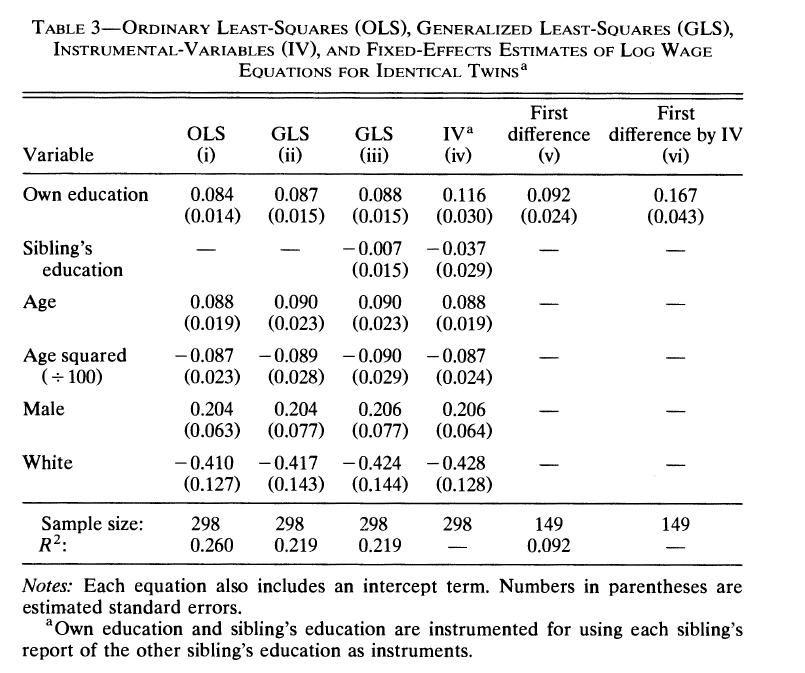
\includegraphics[width=9cm, height=9cm, keepaspectratio]{Figuras/ashenfelter-krueger-gemelos.png}
	\end{figure} 
\end{frame}


%%%%%%%%%%%%%%%%%%%%%%%%%%%%%%%%%%%%%%%%%%%%%%%%%%%%%%%%%%%%%%%%%%%%%
%%%%%%%%%%%%%%%%%%%%%%%%%%%%%%%%%%%%%%%%%%%%%%%%%%%%%%%%%%%%%%%%%%%%%
\section{Modelo de diferencias en diferencias (Cont.)}


\begin{frame}{Modelo de DiD  (Cont.)}
\begin{itemize}\setlength{\itemsep}{1.0em}
	\item El modelo de \textcolor{blue}{diferencias en diferencias} (DiD) se puede plantear, \textcolor{red}{\textbf{bajo ciertas condiciones}}, como un modelo de \textit{TWFE}. 
	%%\pause
	\item \textbf{Notación}:
    \begin{itemize}\setlength{\itemsep}{0.5em}
        \item \(t \in \{0,1,\ldots,T\}\): índice de periodos.
        \item \(i \in \{1,\ldots,N\}\): índice de unidades.
        \item \(\textcolor{red}{t_0} \in \{1,\ldots,T\}\): periodo en el que inicia el tratamiento. Asumimos (por ahora):
    \begin{itemize}
        \item[i)] \textbf{Estado absorbente}: una vez tratada, la unidad permanece tratada.
        \item[ii)] \textbf{Tratamiento simultáneo}: todas las unidades tratadas comienzan en \(\textcolor{red}{t_0}\). %%%\pause
    \end{itemize}
        \item \(D_i \in \{0,1\}\): indicador de pertenencia al grupo tratado.
        \item \(D_{it} = D_i \cdot \mathbf{1}\{t \ge \textcolor{red}{t_0}\}\): indicador \textit{post} para unidades tratadas.
    \end{itemize}	
\end{itemize}	
\end{frame}


\begin{frame}[plain]
    \begin{tcolorbox}[colback=white, title=Diseño de investigación (causal), arc=0mm, boxrule=0.5pt, breakable]
        Declaración estadística y/o económica de cómo se estimará una relación entre dos (o más) variables que es de \textbf{naturaleza causal}.
    \end{tcolorbox}
    %%\pause
    \vspace{1em}
    \begin{itemize}\setlength{\itemsep}{1.0em}
        \item Los diseños pueden clasificarse en dos enfoques:
        \begin{itemize}    
            \item \textcolor{blue}{Basado en la asignación}: el \textbf{estimando} se identifica a partir de supuestos sobre el mecanismo de asignación del tratamiento (e.g., experimentos controlados). %%\pause
            \vspace{0.5em}
            \item \textcolor{blue}{Basado en modelos}: el \textbf{estimando} se identifica modelando los resultados potenciales. %%\pause 
        \end{itemize}
        \item Para pensar en las extensiones de DiD, vamos a tomar un enfoque \textcolor{blue}{basado en modelos} a partir de los supuestos de identificación. 
    \end{itemize}    
\end{frame}


\begin{frame}{Tendencias paralelas}
\begin{itemize}\setlength{\itemsep}{1.0em}
    \item \textbf{\textcolor{blue}{Tendencias paralelas (S1)}}: En \textcolor{red}{\textbf{ausencia de tratamiento}}, los grupos tratado y control siguen la \textbf{misma evolución temporal} (pueden diferir en niveles, pero no en su tendencia).
    %%\pause
    \begin{align*}
        \EX[Y_{it}(0) \mid D_i] = \phi_t + \eta_i \qquad \forall t, \;\; D_i \in \{0,1\}.
    \end{align*}
    \vspace{-1em}
    \begin{itemize}
        \item $\phi_t$ es la \textbf{tendencia común de tiempo}.
        \item $\eta_i$ es un efecto fijo de unidad (o de grupo). Captura las \textbf{diferencias sistemáticas} que son constantes en el tiempo.
    \end{itemize}
    %%\pause
    \smallspace
    \item[$\implies$] $\EX[Y_{it}(0)]$ se descompone aditivamente en un \textbf{efecto fijo de unidad} y un \textbf{efecto fijo de tiempo}.
\end{itemize}	
\end{frame}


\begin{frame}{No anticipación y SUTVA}
\begin{itemize}\setlength{\itemsep}{1.0em}
    \item \textcolor{blue}{\textbf{No anticipación (S2)}}: \\
    \vspace{0.5em}
    \textbf{Para todo \(t<\red{t_0}\)}, no hay efecto del tratamiento:
    \begin{align*}
        Y_{it}(1)=Y_{it}(0) = Y_{it} \quad\Longrightarrow\quad \EX\!\big[Y_{it}\mid D_i\big]=\EX\!\big[Y_{it}(0)\mid D_i\big].
    \end{align*}
    En palabras: antes de la implementación (\(\red{t_0}\)), los resultados potenciales con y sin tratamiento coinciden.
    %%\pause
    \item \textcolor{blue}{\textbf{SUTVA (S3)}}:
    \vspace{-1em}
    \begin{align*}
        Y_{it}(D_i, \mathbf{D_{-i}}) = Y_{it}(D_i)
    \end{align*}
    donde $\mathbf{D_{-i}}$ denota el vector de asignaciones de todas las demás unidades. \\
    \textbf{En palabras}: el resultado de la unidad \(i\) depende únicamente de su propia asignación (sin \textit{spillovers} o interferencia).
\end{itemize}	    
\end{frame}


\begin{frame}{Modelo con efectos constantes y homogéneos}
\begin{itemize}\setlength{\itemsep}{1.0em}
    \item Considere (por ahora) el caso más sencillo con \textcolor{blue}{efectos constantes y homogéneos}: 
    \vspace{-0.5em}
    \begin{align*}
        \EX[Y_{it}(1) -Y_{it}(0) \mid D_{i} = 1] = \textcolor{brown}{\tau}, \quad \forall \, t\geq\red{t_0}.   
    \end{align*}
    %%\pause
    \item \textbf{Combinando S1–S3 y homogeneidad:}
    \begin{align*}
    \begin{split}
        \EX[Y_{it} \mid D_{it} = 1] &= \EX[Y_{it}(0) \mid D_{it} = 1] + \textcolor{brown}{\tau} \\ &= \phi_t + \eta_i + \textcolor{brown}{\tau}.
    \end{split}
    \end{align*}
    Recordar que \(D_{it} = D_i \cdot \mathbf{1}\{t \ge \textcolor{red}{t_0}\}\).
    %%\pause
    \item \textbf{Para \(D_{it} = 0\)},
    \begin{align*}
    \begin{split}
        \EX[Y_{it} \mid D_{it} = 0] &= \EX[Y_{it}(0) \mid D_{it} = 0] = \phi_t + \eta_i.
    \end{split}
    \end{align*}
\end{itemize}	    
\end{frame}


\begin{frame}{Modelo \textit{TWFE}}
\begin{itemize}
    \item \textbf{Representación TWFE de la CEF bajo S1-S3}:
    \begin{align*}
    \begin{split}
        \EX[Y_{it} \mid D_{it}]  &= \phi_t + \eta_i + \textcolor{brown}{\tau} D_{it}.
    \end{split}
    \end{align*}
    %%\pause
    \item \textbf{Por las propiedades de la CEF}:
    \begin{align*}
    \begin{split}
        Y_{it}  &= \phi_t + \eta_i + \textcolor{brown}{\tau} D_{it} + e_{it}, \quad \text{donde } \; \EX[e_{it} \mid D_{it}] = 0.
    \end{split}
    \end{align*}
    Se desprende que \(\plim \textcolor{brown}{\hat \tau_{TWFE}} = \textcolor{brown}{\tau}\).
\end{itemize}	
\end{frame}


\begin{frame}{\textit{TWFE} y DiD}
\begin{itemize}\setlength{\itemsep}{1.0em}
    \item Bajo S1–S3 y efectos homogéneos (\(\brown{\tau}\)), para dos unidades \(i\) (tratada) y \(j\) (control), y para \(k,h\in\mathbb{N}^{+}\):
    \vspace{0.5em}
    \begin{enumerate}\setlength{\itemsep}{0.5em}
        \item \(\EX\!\big[Y_{i,\,\red{t_0}+k}\mid D_i=1\big]=\phi_{\red{t_0}+k}+\eta_i+\textcolor{brown}{\tau}\) %%\pause
        \item \(\EX\!\big[Y_{i,\,\red{t_0}-h}\mid D_i=1\big]=\phi_{\red{t_0}-h}+\eta_i\) %%\pause
        \item \(\EX\!\big[Y_{j,\,\red{t_0}+k}\mid D_j=0\big]=\phi_{\red{t_0}+k}+\eta_j\) %%\pause
        \item \(\EX\!\big[Y_{j,\,\red{t_0}-h}\mid D_j=0\big]=\phi_{\red{t_0}-h}+\eta_j\) %%\pause
    \end{enumerate}    
    \vspace{0.9em}
    \item \textbf{Diferencias en diferencias:}
        \begin{align*}
    \textcolor{brown}{\tau} = \Big((1)-(2)\Big) - \Big((3)-(4)\Big) = \textcolor{brown}{\tau_{\text{DiD}}}
\end{align*}
\end{itemize}
\end{frame}


\begin{frame}{Efectos dinámicos (1)}
\begin{itemize}\setlength{\itemsep}{1.0em}
    \item[1.] \textcolor{blue}{Efectos dinámicos (post)}. Defina el tiempo relativo \(j \equiv t-\red{t_0}\).
    Para \(j \ge 0\) (periodos post):
    \[
        \textcolor{brown}{\tau_j} = \EX \big[ Y_{it}(1)-Y_{it}(0) | D_i=1, t= j + \red{t_0}\big].
    \]
    \textcolor{red}{Intuición}: \(\textcolor{brown}{\tau_j}\) es el efecto promedio \(j\) periodos después de la implementación. %%\pause
    \item Podemos extendernos a un \textbf{modelo dinámico} de la forma:
    \begin{align*}
        Y_{it} = \phi_t + \eta_i + \sum_{j=0}^{T - \textcolor{red}{t_0}} \textcolor{brown}{\tau_j} D_i \mathbf{1}\{j=t-\textcolor{red}{t_0}\} + e_{it}.
    \end{align*}        
    Hay un efecto estimado para cada periodo relativo \(j \geq 0\).
\end{itemize}
\end{frame}


\begin{frame}{Efectos dinámicos (2)}
    \begin{itemize}\setlength{\itemsep}{1.0em}
        \item[2.] \textcolor{blue}{Efectos dinámicos (pre)}. Para \(j < 0\) (periodos pre):
        \[
        \textcolor{brown}{\tau_j} = \EX[Y_{it}(1)- Y_{it}(0) \mid D_{i}, t= j + \red{t_0}] = 0.
        \]
        \textcolor{red}{¿Por qué?} \textcolor{red}{¿Qué implica que \(\textcolor{brown}{\tau_j} \neq 0\) para \(j < 0\)?}
        %%\pause
        \item Considere el \textbf{modelo dinámico} ampliado:
		\begin{align*}
			Y_{it} = \phi_t + \eta_i + \sum_{j \neq -1} \textcolor{brown}{\tau_j} D_i \mathbf{1}\{j=t-\textcolor{red}{t_0}\} + e_{it}.
		\end{align*}
        Se debería cumplir que \(\textcolor{brown}{\tau_j} = 0\) para \(j < -1\).
        \vspace{0.5em}
        %%\pause
        \begin{itemize}\setlength{\itemsep}{0.3em}
            \item Tenemos que elegir un periodo de referencia previo a la implementación del tratamiento (e.g., $j = - 1$) \textcolor{red}{¿Por qué?} \textcolor{red}{¿Importa qué periodo?} %%%\pause
            \item Los efectos se interpretan relativo a la diferencia (tratamiento vs. control) en ese periodo.
        \end{itemize}
    \end{itemize}   
\end{frame}


\begin{frame}{Modelo \textit{TWFE} con efectos dinámicos y heterogéneos}
    \begin{itemize}\setlength{\itemsep}{1.0em}
    \item[3.] Con \textcolor{blue}{efectos heterogéneos} (\(\textcolor{brown}{\tau_{ij}}\)), los parámetros \(\textcolor{brown}{\tau_{j}}\) del \textbf{modelo dinámico} (o el \(\textcolor{brown}{\tau}\) del \textbf{modelo estático}) se pueden interpretar como un promedio ponderado en cada tiempo relativo:
    \[
    \textcolor{brown}{\tau_j} = \EX[\textcolor{brown}{\tau_{ij}} \mid D_{i}, t= j + \red{t_0}].
    \]
    donde los pesos están dados por la forma del estimador MCO (recordar diapositivas de \textit{matching}). %%\pause
    \item \textcolor{red}{\textbf{Importante}}: esto no aplica para \textcolor{blue}{estudio de eventos} donde \(\textcolor{red}{t_0}\) puede variar entre cohortes.
    \end{itemize}   
\end{frame}

% \begin{frame}{Modelo TWFE: Extensiones}
% \begin{itemize}
%     \item Suponga que en ausencia de tratamiento, las tendencias difieren según unas características $\xB_{it}$ observables:
%     \begin{align*}
%         \EX[Y_{it}(0)] = \eta_i + \underbrace{\phi_t + \xB'_{it}\betaB}_{\text{Tendencia}} \;\; \text{para} \;\; D_i \in \{0,1\}.
%     \end{align*}        
%     Bajo los supuestos descritos, el \textbf{modelo estático} es:
%     \begin{align*}
%         Y_{it} = \eta_i + \phi_t  + \textcolor{brown}{\tau} D_{it} + \xB'_{it}\betaB + \epsilon_{it}.
%     \end{align*}
% %%%%%\pause
%     \item Suponga que $D_{it}$ no es binaria. Por ejemplo, si $D_i \in \{0, 1 \ldots, J\}$ y los efectos son lineales:
%     \begin{align*}
%         \EX[y^d_{dt} -Y_{it}(0)] = \textcolor{brown}{\tau} d \;\; \forall \;\; t \geq \red{t_0}.
%     \end{align*}
%     Llegamos al mismo modelo de regresión, pero la interpretación cambia.
% \end{itemize}
% \end{frame}

%%%%%%%%%%%%%%%%%%%%%%%%%%%%%%%%%%%%%%%%%%%%%%%%%%%%%%%%%%%%%%
%%%%%%%%%%%%%%%%%%%%%%%%%%%%%%%%%%%%%%%%%%%%%%%%%%%%%%%%%%%%%%
\section{Supuesto de tendencias paralelas}

\begin{frame}{Supuesto de tendencias paraleles}
\begin{itemize}\setlength{\itemsep}{1.0em}
	\item El supuesto de \textcolor{blue}{tendencias paralelas} se puede validar \textbf{parcialmente} si tenemos datos para varios \textbf{periodos pretratamiento}.
    %%\pause
	\smallspace
	\item \textcolor{red}{\textbf{Intuición}}: la diferencia entre las unidades tratadas y de control en cualquier período previo al tratamiento es constante. Si el modelo es:
    \begin{align*}
        Y_{it} = \phi_t + \eta_i + \sum_{j \neq -1} \textcolor{brown}{\tau_j} D_i \mathbf{1}[j=t-\textcolor{red}{t_0}] + e_{it},
    \end{align*}
    se debería cumplir que \(\textcolor{brown}{\tau_j} = 0\) para \(j < -1\).      	
\end{itemize}
\end{frame}


\begin{frame}{Representación gráfica (1)}
	\begin{itemize}
		\item Suponga que usted hace una figura con el promedio de \(Y\) para ambos grupos \(D \in \{0,1\}\): \\ \vspace{0.1cm}
	\begin{center}
	\begin{tikzpicture}[scale=0.45]
	\draw[thick,<->] (-3,7) node[above]{$\EX[Y|D]$}--(-3,0)--(15,0) node[right]{$j$};
	\draw (-2,3) -- (2,1) -- (6,2.5) -- (10,2) --(14,2.2) node[right]{\tiny Tratamiento (\(D=1\))};
	\draw[blue, dashed] (10,2) --(14,5) node[right]{\tiny Contrafactual};	
	\draw[fill] (10,2) circle [radius =0.2];			
	\draw[fill] (14,2.2) circle [radius =0.2];
	\draw[red,fill] (14,6) circle [radius =0.2];		
	\draw[red] (-2,4) -- (2,2) -- (6,3.5) -- (10,3) --(14,6) node[right]{\tiny Control (\(D=0\))};
	\draw[red,fill] (10,3) circle [radius =0.2];			
	\draw[blue, fill] (14,5) circle [radius =0.2];	
	\draw [dotted, thick] (12,0)--(12,7);
  	\draw[red,fill] (-2,4) circle [radius =0.2];
   \draw[fill] (-2,3) circle [radius =0.2];
	\draw[fill] (2,1) circle [radius =0.2];			
	\draw[fill] (6,2.5) circle [radius =0.2];
	\draw[red,fill] (2,2) circle [radius =0.2];			
	\draw[red,fill] (6,3.5) circle [radius =0.2];	
	%	\node [below] at (8,0) {Intervención};
    \node [below] at (-2,0) {$-4 $};
    \node [below] at (2,0) {$-3$};
    \node [below] at (6,0) {$-2$};
    \node [below] at (10,0) {$-1$};
    \node [below] at (14,0) {$0$};		
	\end{tikzpicture}
\end{center}  
    donde $j= t - \red{t_0}$. ¿Se cumple el supuesto de tendencias paralelas \textbf{pretratamiento}?
	\end{itemize}	
\end{frame}

\begin{frame}{Representación gráfica (2)}
\begin{itemize}
	\item Suponga ahora que usted observa: \\ \vspace{0.1cm}
	\fontvie
	\begin{center}
		\begin{tikzpicture}[scale=0.45]
		\draw[thick,<->] (-3,7) node[above]{$\EX[y|D]$}--(-3,0)--(15,0) node[right]{$j$};
		\draw (-2,3) -- (2,1) -- (6,2.5) -- (10,2) --(14,2.2) node[right]{\tiny Tratamiento};
		\draw[blue, dashed] (10,2) --(14,5) node[right]{\tiny Contrafactual};	
		\draw[fill] (10,2) circle [radius =0.2];			
		\draw[fill] (14,2.2) circle [radius =0.2];
		\draw[red,fill] (14,6) circle [radius =0.2];		
		\draw[red] (-2,5) -- (2,7) -- (6,4) -- (10,3) --(14,6) node[right]{\tiny Control};
		\draw[red,fill] (10,3) circle [radius =0.2];			
		\draw[blue, fill] (14,5) circle [radius =0.2];	
		\draw [dotted, thick] (12,0)--(12,7);	
  	\draw[fill] (-2,3) circle [radius =0.2];	
		\draw[fill] (2,1) circle [radius =0.2];			
		\draw[fill] (6,2.5) circle [radius =0.2];
  	\draw[red,fill] (-2,5) circle [radius =0.2];
		\draw[red,fill] (2,7) circle [radius =0.2];			
		\draw[red,fill] (6,4) circle [radius =0.2];	
		%	\node [below] at (8,0) {Intervención};
        \node [below] at (-2,0) {$-4$};
        \node [below] at (2,0) {$-3$};
        \node [below] at (6,0) {$-2$};
		\node [below] at (10,0) {$-1$};
		\node [below] at (14,0) {$0 $};		
		\end{tikzpicture}
	\end{center}
\vspace{0.2cm}
donde $j= t - \red{t_0}$. ¿Se cumple el supuesto de tendencias paralelas \textbf{pretratamiento}?
\end{itemize}	
\end{frame}


\begin{frame}{Ejemplo 1: Movilidad durante la pandemia (tendencias)}
	\begin{figure}[H]
		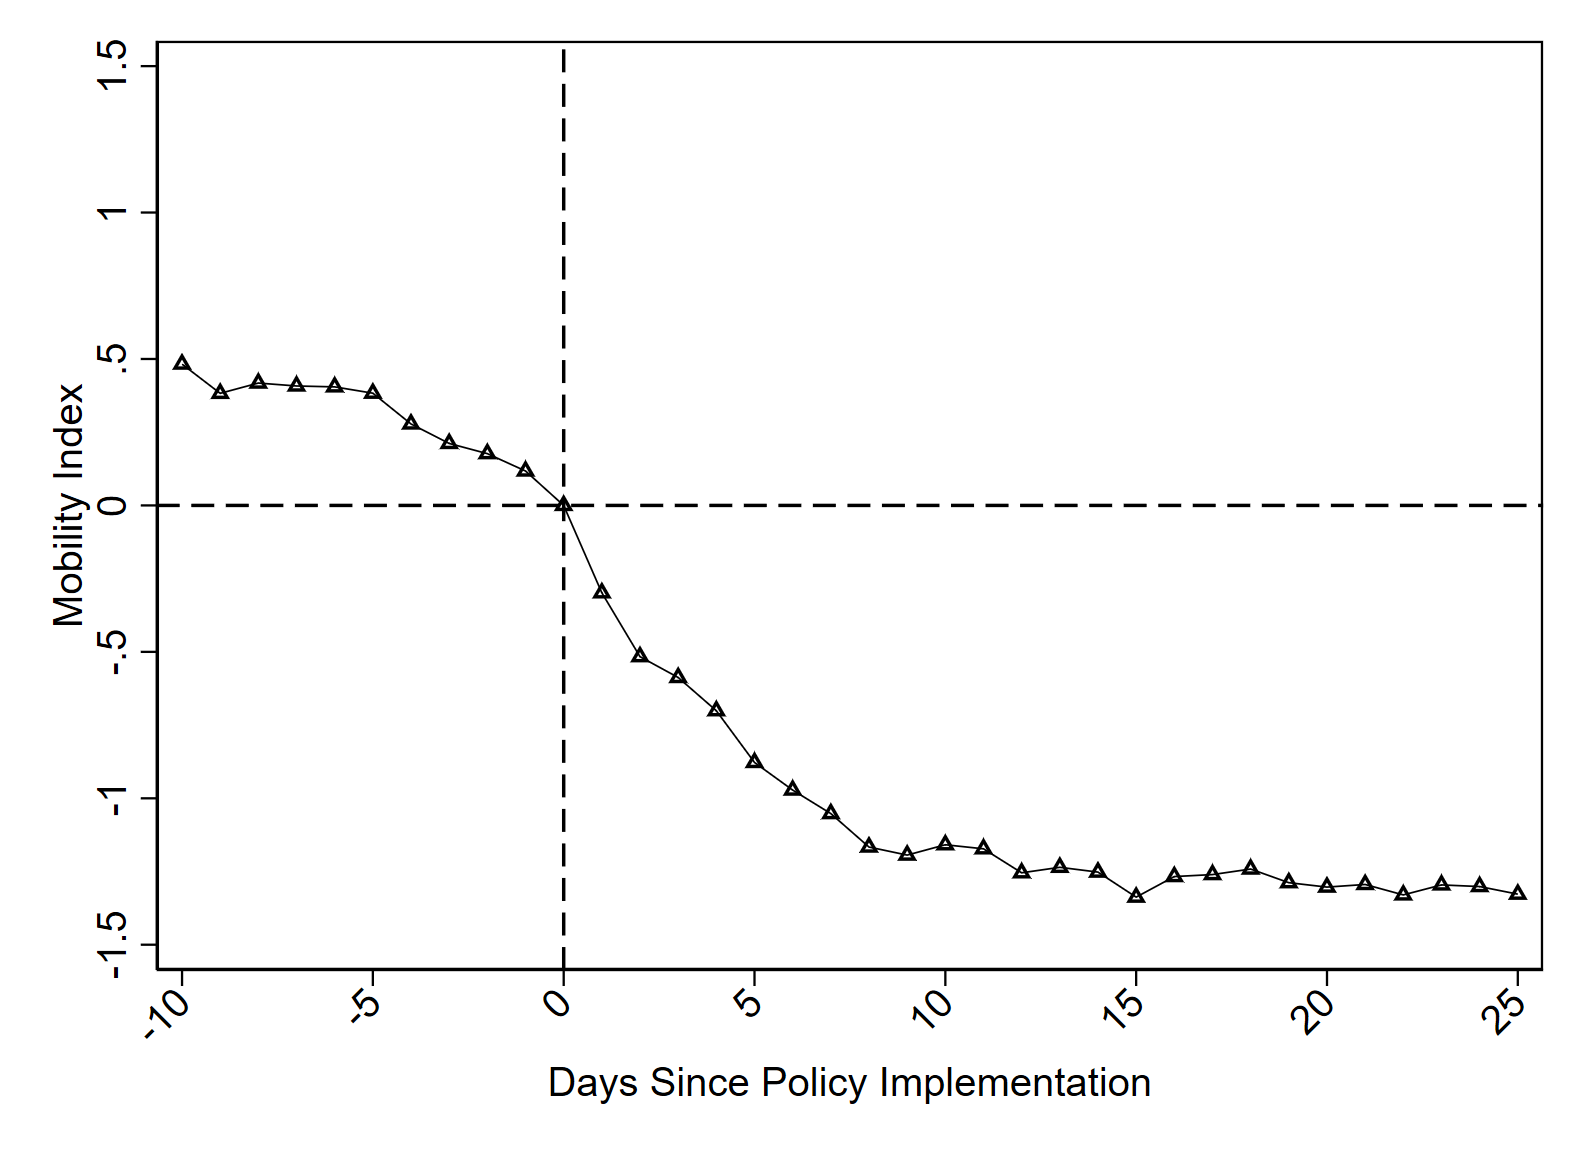
\includegraphics[width=9cm, height=9cm, keepaspectratio]{Figuras/movilidad-pandemia-tendencias.png}
	\end{figure}
\end{frame}


\begin{frame}{Ejemplo 1: Movilidad durante la pandemia (modelo dinámico)}
	\begin{figure}[H]
		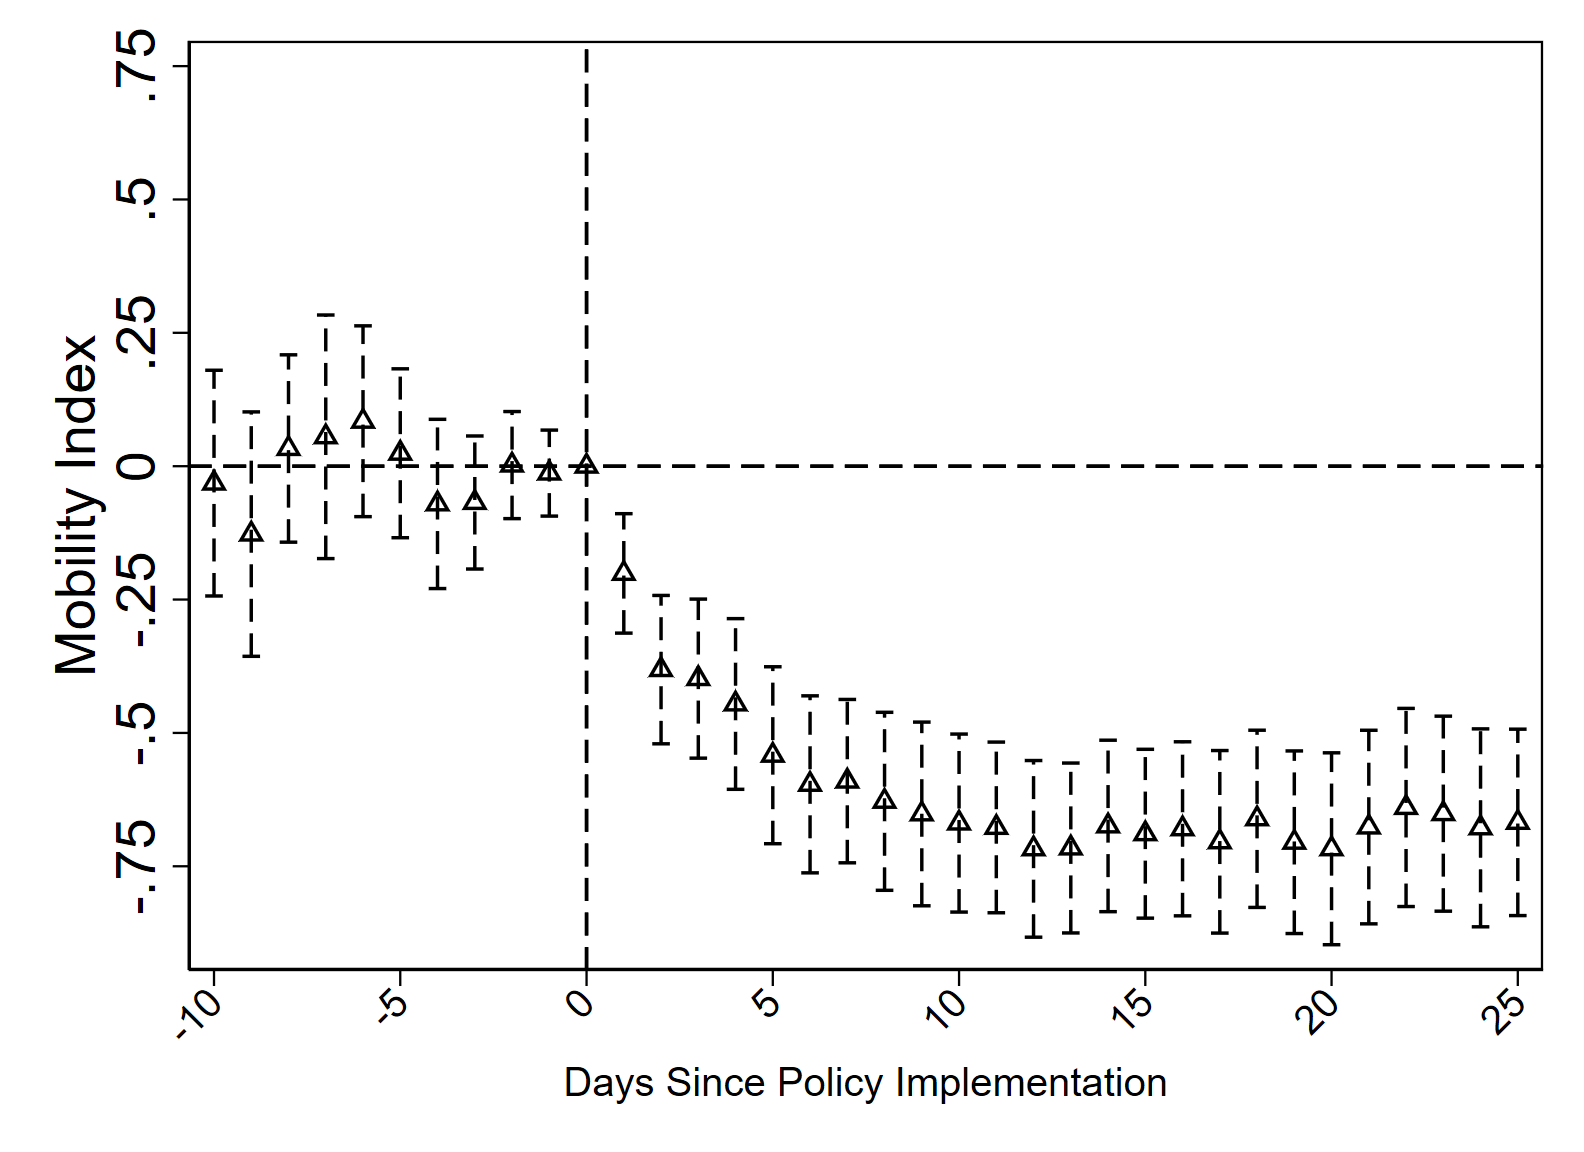
\includegraphics[width=9cm, height=9cm, keepaspectratio]{Figuras/movilidad-pandemia-modelo-dinamico.png}
	\end{figure}
\end{frame}


\begin{frame}{Ejemplo 2: coca y PNIS (modelo dinámico)}
   \begin{figure}
        \centering
        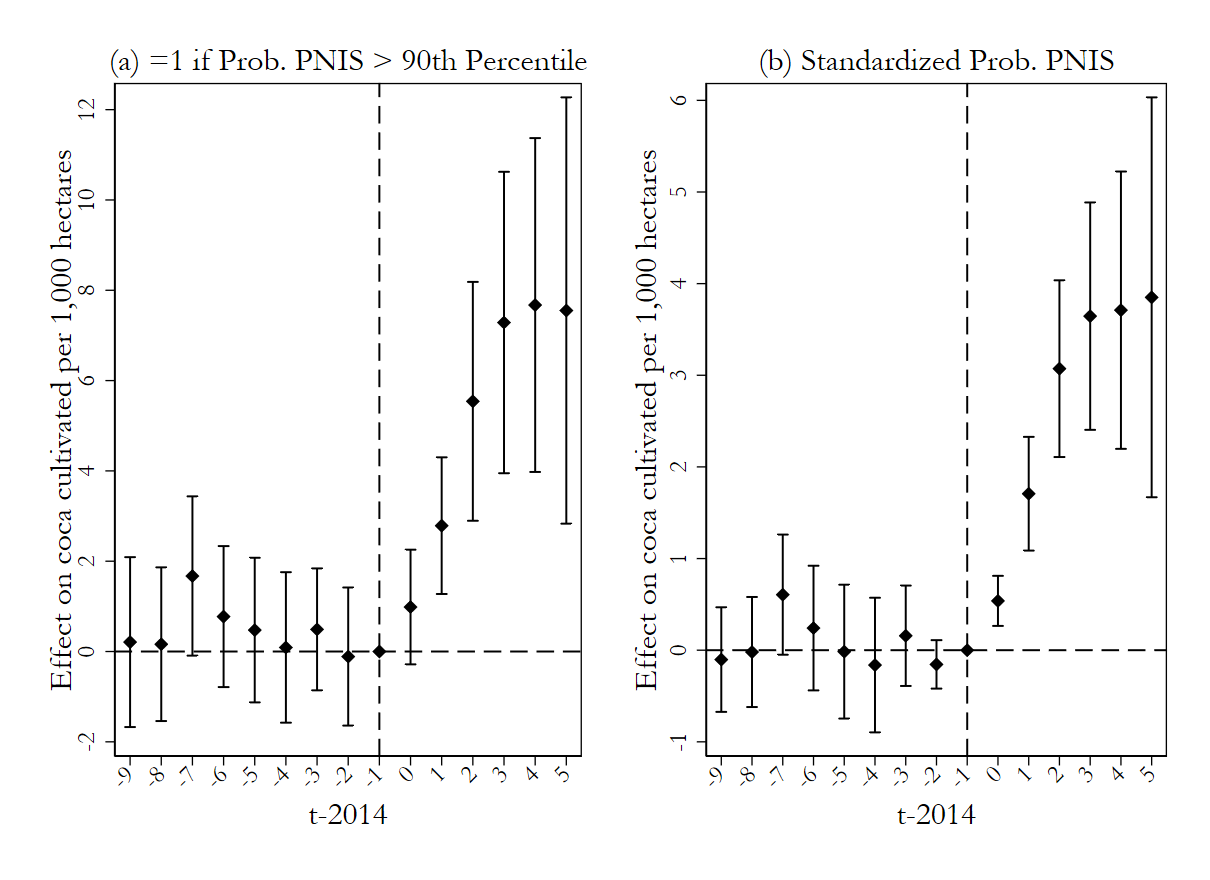
\includegraphics[width=0.95\linewidth]{Figuras/coca-pnis-modelo-dinamico.png}
    \end{figure} 
\end{frame}

%%%%%%%%%%%%%%%%%%%%%%%%%%%%%%%%%%%%%%%%%%%%%%%%%%%%%%%%%%%%%%
%%%%%%%%%%%%%%%%%%%%%%%%%%%%%%%%%%%%%%%%%%%%%%%%%%%%%%%%%%%%%%
\section{Cambios en la composición y formas funcionales}

\begin{frame}{Cambios en la composición}
\begin{itemize}
	\item El tratamiento puede \textbf{cambiar la composición} de los grupos.
	\smallspace
	%%\pause
	\item Suponga que un departamento diseña una política de transferencias condicionales para ayudar a la población migrante.
	\smallspace
	\begin{enumerate}
		\item Induce a ciertas personas a trasladarse a este departamento.
		\smallspace
		\item Las personas que se mueven son (potencialmente) diferentes a los que se quedan.
		\smallspace
	\end{enumerate}
	%%\pause
	\item Incluso si la política no tiene ningún efecto real, la composición de la muestra en cada grupo puede cambiar, lo que puede generar efectos espurios.
\end{itemize}	
\end{frame}


\begin{frame}{Forma funcional}
\begin{itemize}
	\item El cumplimiento del supuesto de \textbf{tendencias paralelas} puede depender de la forma funcional con la que modelamos la variable de resultado.
	\smallspace
	%\pause
	\item Considere los siguientes modelos:
	\begin{align*}
	Y_{it} = \phi_t + \eta_i + \textcolor{brown}{\tau} D_{it} + e_{it},
	\end{align*}
	\vspace{-2em}
	\begin{align*}
	\ln Y_{it} = \phi_t + \eta_i + \textcolor{brown}{\tau} D_{it} + e_{it}.
	\end{align*}
	\vspace{-0.5cm}
	%\pause
	\item Suponga que el tratamiento corresponde a un programa de empleo, con los siguientes cambios observados:
	\smallspace
    \begin{itemize}
        \item El empleo sube de 20\% a 30\% para el grupo tratado.
        \item El empleo sube de 5\% a 10\% para el grupo de control. %\pause
        \item \textcolor{red}{Efecto DiD (niveles)}: aumento de 5 puntos porcentuales. %\pause
        \item \textcolor{red}{Efecto DiD (logaritmos)}: 
        \[
        [\ln(30) - \ln(20)] - [\ln(10) - \ln(5)] = \ln(1.5) - \ln(2) < 0.
        \]
    \end{itemize}    
\end{itemize}
\end{frame}

%%%%%%%%%%%%%%%%%%%%%%%%%%%%%%%%%%%%%%%%%%%%%%%%%%%%%%%%%%%%%%
%%%%%%%%%%%%%%%%%%%%%%%%%%%%%%%%%%%%%%%%%%%%%%%%%%%%%%%%%%%%%%
\section{Modelo de diferencias en diferencias en diferencias (DDD)}

\begin{frame}{Modelo de diferencias en diferencias en diferencias (DDD)}
\begin{itemize}\setlength{\itemsep}{1.0em}
	\item Cuando no se cumple \textcolor{blue}{tendencias paralelas}, una tercera diferencia puede ayudar con la identificación.
	%\pause
	\item Ejemplo: \citet{muralidharan2017cycling}: 
	\smallspace
	\begin{itemize}\setlength{\itemsep}{0.3em}
		\item En el estado de Bihar, India, se diseñó una intervención para reducir la brecha entre hombres y mujeres en la cobertura de educación secundaria.
		\item Las \textbf{mujeres} que permanecían en la escuela \textbf{recibían una bicicleta} que les facilitaba trasladarse al colegio, reduciendo el costo de movilidad.
		\item \textbf{Los hombres} no recibían nada.
	\end{itemize}
\end{itemize}	
\end{frame}


\begin{frame}{Especificación DiD}
\begin{itemize}\setlength{\itemsep}{1.0em}
    \item Una posibilidad es estimar un modelo de DiD comparando la tasa de cobertura de las mujeres antes y después del tratamiento, usando a los hombres en las mismas cohortes como grupo de control.
    %\pause
    \smallspace
    \begin{align*}
        y_{gt} = \beta_0 + \beta_1 \text{Post}_t + \beta_2 \text{Mujer}_g + \textcolor{brown}{\beta_3} (\text{Post}_t \times \text{Mujer}_g) + e_{gt},
    \end{align*}
    donde:
    \begin{itemize}
        \item $g$ indexa el sexo (hombre/mujer),
        \item $t$ indexa el período (pre/post),
        \item $y_{gt}$ es la tasa de cobertura en el estado de Bihar para el grupo $g$ en el período $t$.
    \end{itemize}
    %\pause
    \item El coeficiente \(\textcolor{brown}{\beta_3}\) estima el efecto a través de una comparación por DiD.
\end{itemize}
\end{frame}


\begin{frame}{¿Una nueva diferencia?}
\begin{itemize}\setlength{\itemsep}{1.0em}
	\item \textbf{Problema:} hombres y mujeres pueden presentar \textcolor{red}{\textbf{tendencias distintas}} en las tasas de cobertura; es decir, la brecha de género podría no ser constante en el tiempo.
	%\pause
	\item Sin embargo, es razonable suponer que dicha brecha sigue una trayectoria similar en estados no tratados: esto implica \textcolor{blue}{tendencias paralelas} en la \textcolor{blue}{brecha de género} entre estados en \textcolor{red}{\textbf{ausencia del tratamiento}}.
    %\pause
	\begin{align*}
	DDD = DiD_{Bihar} - DiD_{Jharkhand}
	\end{align*}
    \vspace{-1em}
        \begin{itemize}
    	\item $DiD_{Bihar}$: Efecto causal $+$ cambio en la brecha de género.
    	\item $DiD_{Jharkhand}$: Cambio en la brecha de género.
        \end{itemize}    
\end{itemize}	
\end{frame}


\begin{frame}{Especificación DDD}
\begin{itemize}\setlength{\itemsep}{1.0em}   
    \item Modelo extendido con una \textbf{tercera diferencia} (estado, período, género):
    \begin{align*}
    \begin{split}
    y_{sgt} =\; & \beta_0 + \beta_1 \text{Bihar}_s + \beta_2 \text{Post}_t + \beta_3 \text{Mujer}_g \\
    & + \beta_4 (\text{Bihar}_s \times \text{Mujer}_g) + \beta_5 (\text{Bihar}_s \times \text{Post}_t) \\
    & + \beta_6 (\text{Post}_t \times \text{Mujer}_g) + \textcolor{brown}{\tau} (\text{Bihar}_s \times \text{Post}_t \times \text{Mujer}_g) + \varepsilon_{sgt}
    \end{split}
    \end{align*}
    %\pause
    \item El coeficiente \(\textcolor{brown}{\tau}\) estima el efecto diferencial del tratamiento sobre las mujeres en Bihar, controlando por diferencias comunes a género, tiempo y estado.
    \item Hay una versión equivalente con efectos fijos. Intente derivarla.
\end{itemize}
\end{frame}


\begin{frame}{Ejemplo: \citet{muralidharan2017cycling} }
		\begin{figure}[H]
			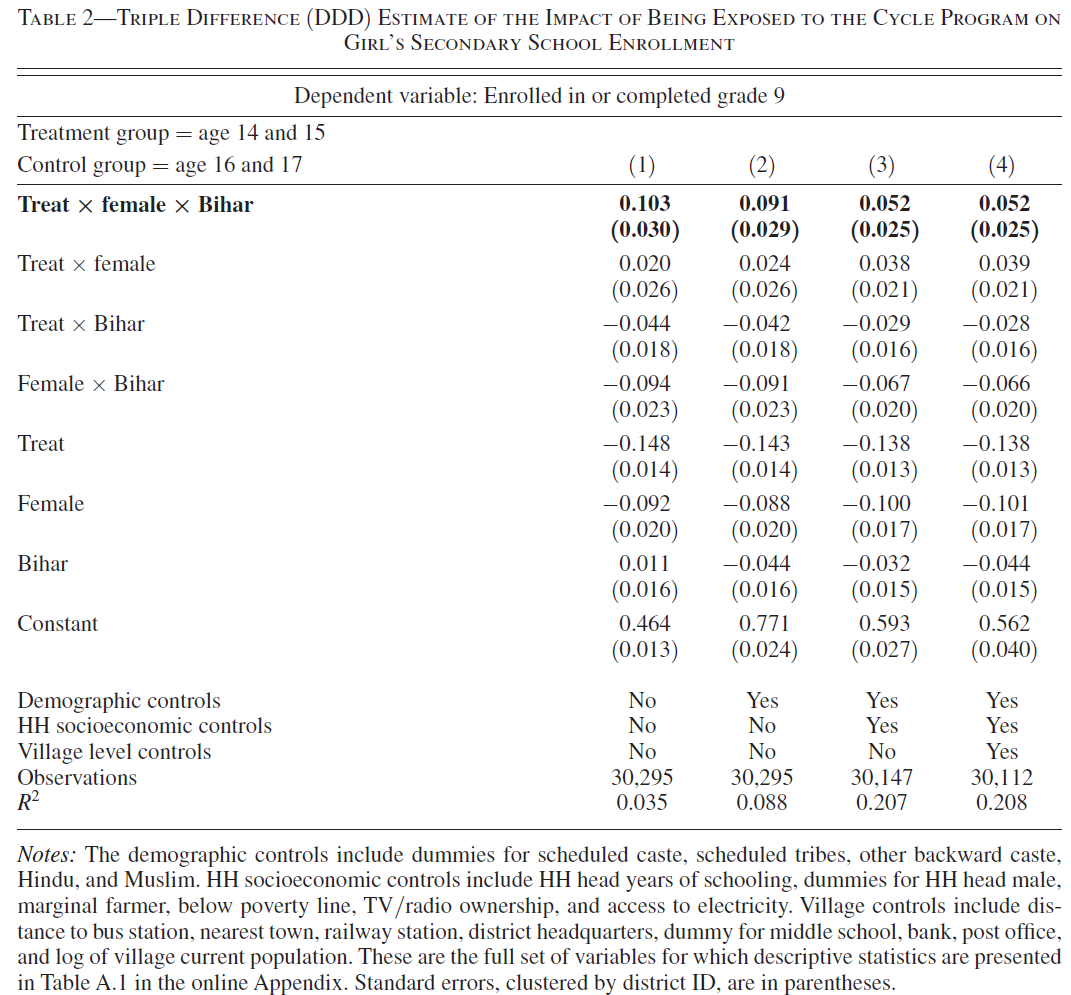
\includegraphics[width=7.5cm, height=7.5cm, keepaspectratio]{Figuras/muralidharan-bihar-ciclos.png}
		\end{figure}    
	\begin{itemize}
	\vspace{-0.5em}
	    \item Resumen del trabajo en este \href{https://www.youtube.com/watch?time_continue=41&v=6nG63ISt_Ek&feature=emb_logo}{enlace}.
	\end{itemize}
\end{frame}


%%%%%%%%%%%%%%%%%%%%%%%%%%%%%%%%%%%%%%%%%%%%%%%%%%%%%%%%%%%%%%
%%%%%%%%%%%%%%%%%%%%%%%%%%%%%%%%%%%%%%%%%%%%%%%%%%%%%%%%%%%%%%
\section{Estudio de eventos}


\begin{frame}{Estudio de eventos}
\begin{itemize}\setlength{\itemsep}{1.0em}  
    \item Un \textcolor{blue}{estudio de eventos} (diseño escalonado) es una generalización de \textcolor{blue}{diferencias en diferencias} cuando las unidades pueden recibir el tratamiento en diferentes momentos del tiempo. %\pause
	\item \textbf{Notación (adicional)}:
    \vspace{0.3em}
    \begin{itemize}\setlength{\itemsep}{0.3em}
        \item \(G_i = \min\{t : D_{it} = 1\}\): el primer periodo en el que la unidad \(i\) recibe tratamiento.
        \vspace{0.3em}
        \begin{itemize}\setlength{\itemsep}{0.1em}
            \item[i)] \textbf{Estado absorbente}: una vez tratada, la unidad permanece tratada.
            \item[ii)] Si la unidad nunca es tratada, usamos \(G_i = \infty\).
            \item[iii)] Todas las unidades que comparten un mismo \(G_i\) hacen parte de la misma \textcolor{red}{\textbf{cohorte}}.
        \end{itemize}
        %\pause
        \item \(Y_{it}(g)\): resultado potencial de \(i\) en \(t\) si hubiese sido tratada por primera vez en \(G_i = g\).
        \item \(Y_{it}(\infty)\): resultado potencial de \(i\) en \(t\) si nunca hubiese sido tratada (\(G_i = \infty\)).
    \end{itemize}
\end{itemize}
\end{frame}


\begin{frame}{Estimandos más usados}
\begin{itemize}\setlength{\itemsep}{2em}
    \item \textbf{ATT por grupo-periodo (cohorte $G_i = g$, tiempo $t$):}
    \begin{align*}
        \brown{ATT(g,t)} = \EX \big[Y_{it}(g) - Y_{it}(\infty) \mid G_i=g\big].
    \end{align*}
    \vspace{-1.5em}
    %\pause
    \item \textbf{ATT por \emph{tiempo relativo} \(j=t-G_i \geq 0\):}
    \begin{align*}
        \brown{ATT_j^{\omega}} = \sum_{g} \omega_g \brown{ATT(g,g+j)}, \quad \text{con} \;\; \omega_g \geq 0 \;\; \text{y} \;\; \sum_g \omega_g = 1.
    \end{align*}
    \vspace{-1.5em}
    %\pause
    \item \textbf{ATT global (para \(j=t-G_i \geq 0\)):}
    \begin{align*}
        \brown{ATT^{\omega}} = \sum_{j} \sum_g \omega_{g,j} \brown{ATT(g,g+j)}, \quad \text{con} \;\; \omega_{g,j} \geq 0 \;\; \text{y} \;\; \sum_{j} \sum_g \omega_{g,j} = 1.
    \end{align*}
\end{itemize}
\end{frame}


\begin{frame}{Cambios en los supuestos}
\begin{itemize}\setlength{\itemsep}{1.0em}
    \item \textbf{\textcolor{blue}{Tendencias paralelas generalizadas (S1b)}}: Para todo \(t \neq t'\) y \(g \neq g'\),
    \begin{equation*}
    \EX \left[Y_{it}(\infty) - Y_{it'}(\infty) \mid G_i = g \right]
    =
    \EX \left[Y_{it}(\infty) - Y_{it'}(\infty) \mid G_i = g' \right].
    \end{equation*}
    En palabras, en \textbf{ausencia del tratamiento}, la variación promedio entre \(t\) y \(t'\) sería la misma para cualquier par de cohortes \(g\) y \(g'\) (incluyendo el grupo nunca tratado). 
    %\pause
    \item \textcolor{blue}{\textbf{No anticipación (S2b)}}: \\
    \vspace{0.5em}
    \textbf{Para todo \(t<g\)}, no hay efecto del tratamiento:
    \begin{align*}
        Y_{it}(g)=Y_{it}(\infty).
    \end{align*}
    \vspace{-1.0em}
    %\pause
    \item El supuesto de SUTVA \textcolor{blue}{\textbf{(S3)}} se mantiene igual.
\end{itemize}	
\end{frame}


\begin{frame}{¿El modelo TWFE estático sigue siendo válido?}
\begin{itemize}\setlength{\itemsep}{1.0em}
    \item Considere el \textbf{modelo estático} de TWFE:
	\begin{align*}
	Y_{it} = \phi_t + \eta_i + \textcolor{brown}{\tau^{twfe}} D_{it} + e_{it}.
	\end{align*}
	%\pause
    En \textcolor{blue}{diseños escalonados}, el \textcolor{red}{efecto estimado por MCO (\(\brown{\hat \tau^{twfe}_{mco}}\)) no siempre tiene una interpretación causal ``intuitiva''}, incluso si se cumplen los supuestos descritos. 
    %\pause  
    \item \textbf{Excepcíon}: no hay heterogeneidad en los efectos del tratamiento 
    \vspace{0.3em}
    \begin{enumerate}\setlength{\itemsep}{0.2em}
        \item A lo largo del tiempo (\textcolor{red}{efectos constantes}), %\pause
        \item Entre unidades (\textcolor{red}{efectos homogéneos}). %\pause
    \end{enumerate}
    \vspace{0.5em}
    \[
        \brown{\tau_{it}(g)} \equiv Y_{it}(g) - Y_{it}(\infty) = \brown{\tau}, \qquad \forall i,\, t\geq g.
    \]
    Es difícil argumentar que se cumple en la mayoría de los casos.
\end{itemize}
\end{frame}


\begin{frame}{El problema de los pesos negativos en TWFE}
\begin{itemize}\setlength{\itemsep}{1.0em}
    \item \textcolor{blue}{Sólo heterogeneidad temporal:} el efecto depende del tiempo relativo al evento, pero toda unidad a \(j\) periodos post adopción tiene el mismo efecto \(\brown{\tau_j}\). 
    %\pause
    \item \textbf{TWFE como promedio ponderado:} \citet{DeChaisemartin2020}; \citet{Goodman-Bacon2021} muestran que
    \vspace{0.0em}
    \[
        \brown{\tau^{twfe}} = \sum_j \omega^{twfe}_j \brown{\tau_j},\quad \text{con} \;\; \sum_j\omega^{twfe}_j=1\ \text{pero puede haber } \omega^{twfe}_j<0.
    \]
    \textcolor{red}{\textbf{Pesos pueden ser negativos!}}.  
    %\pause
    \item \textcolor{blue}{Heterogeneidad en tiempo \emph{y} unidades:} \(\brown{\tau_{it}(g)}\) puede recibir \emph{peso negativo} para algunas combinaciones de \(t\) y \(g\).
\end{itemize}
\end{frame}


\begin{frame}{Caracterizando el problema}
    \begin{itemize}
        \item \textbf{Tres cohortes}: nunca-tratados ($G_i=U\equiv \infty$), tratados temprano ($G_i=k$), tratados tarde ($G_i=l$), con $k<l$. 
        \vspace{1em}
        %\pause
        \begin{figure}[H]
            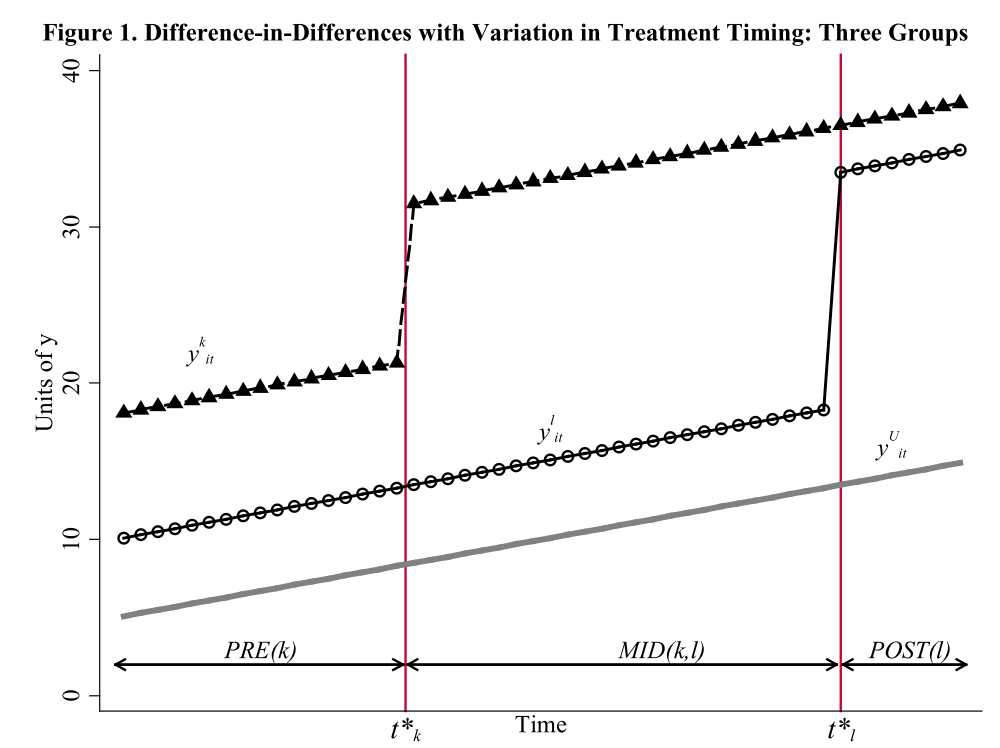
\includegraphics[width=8cm, height=8cm, keepaspectratio]{Figuras/goodman-bacon-cohortes.png}
        \end{figure}
    \end{itemize}
\end{frame}


\begin{frame}{Descomposición de \citet{Goodman-Bacon2021}}
\begin{itemize}\setlength{\itemsep}{1.0em}
    \item El estimador de $\textcolor{brown}{\tau^{twfe}}$ se descompone como un \textbf{promedio ponderado} de todos los posibles estimadores de DiD de 2$\times$2 entre cohortes.
    \vspace{1em}
    \smallspace
    \begin{figure}[H]
        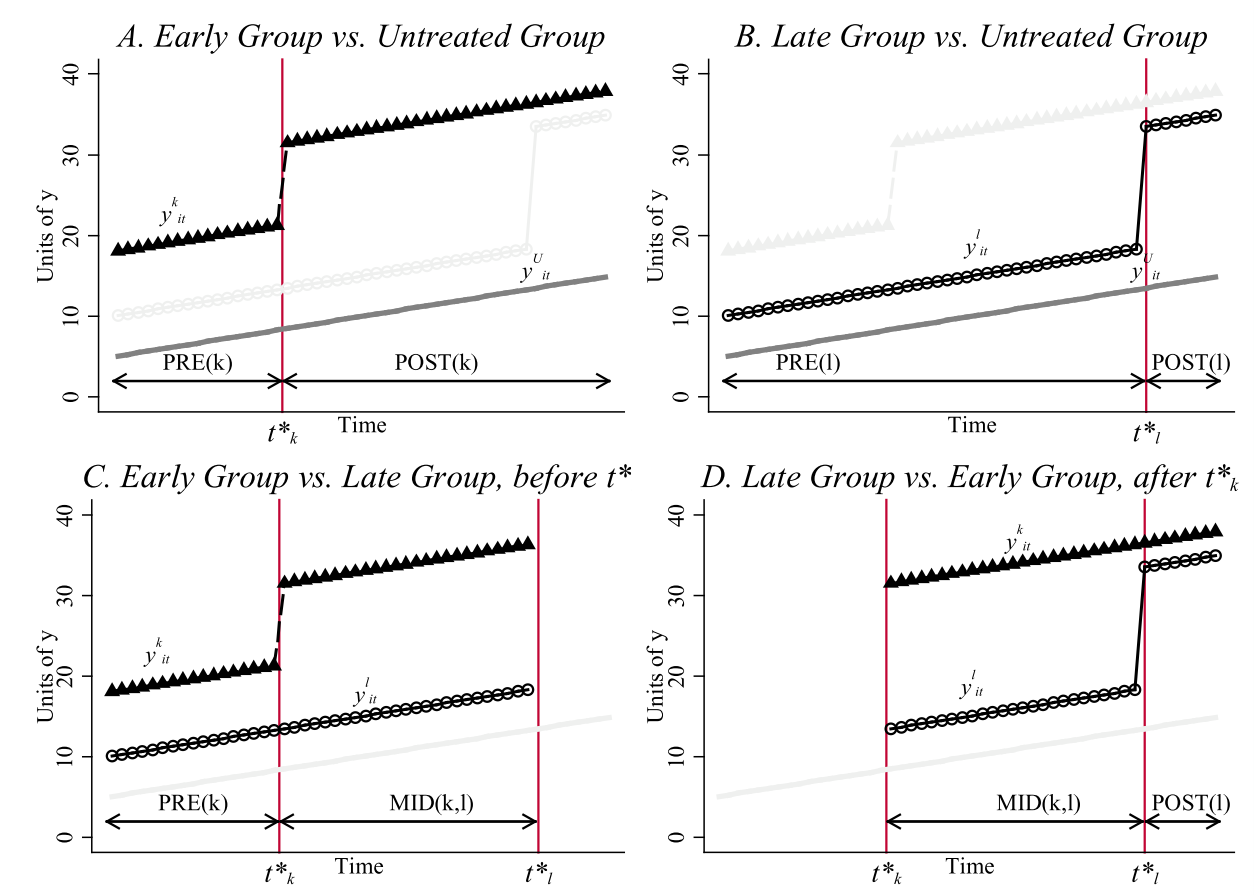
\includegraphics[width=8cm, height=8cm, keepaspectratio]{Figuras/goodman-bacon-descomposicion.png}
    \end{figure}
\end{itemize}
\end{frame}


\begin{frame}{Comparaciones indebidas}
\begin{itemize}\setlength{\itemsep}{0.8em}
    \item \textcolor{red}{\textbf{Comparaciones indebidas}}: en una de las comparaciones DiD \(2\times2\), el grupo tratado \emph{tarde} se compara con el grupo tratado \emph{temprano} \textbf{después} de que éste ya recibió el tratamiento
    \(\Rightarrow\) el contrafactual se construye con unidades ya tratadas.
\end{itemize}
\end{frame}


\begin{frame}{Descomposición del sesgo en TWFE estático}
\begin{itemize}\setlength{\itemsep}{1em}
    \item \textbf{Estimando asintótico \citep{Goodman-Bacon2021}}:
    \[
        \operatorname{plim}_{N\to\infty}\,\brown{\hat\tau^{twfe}_{mco}}
        =
        \underbrace{\text{VWATT}}_{\text{promedio causal}}
        +
        \underbrace{\text{VWCT}}_{\text{falla de tendencias paralelas}}
        -
        \underbrace{\Delta ATT}_{\text{heterogeneidad}}.
    \]
    \begin{enumerate}\setlength{\itemsep}{0.25em}
        \item \textbf{VWATT} (\emph{variance–weighted ATT}): promedio ponderado de los efectos causales. %\pause
        \item \textbf{VWCT} (\emph{variance–weighted common trends}): sesgo si no se cumple \textcolor{blue}{tendencias paralelas generalizadas}. %\pause
        \item \(\boldsymbol{\Delta ATT}\) (\emph{heterogeneity bias}): surge cuando el efecto varía por cohorte o por tiempo relativo (\(t-G_i\)).
    \end{enumerate}
\end{itemize}
\end{frame}


\begin{frame}{¿El modelo TWFE dinámico sigue siendo válido?}
\begin{itemize}\setlength{\itemsep}{0.8em}
    \item \textbf{Especificación dinámica}:
    \begin{align*}
        Y_{it} = \phi_t + \eta_i + \sum_{j\neq -1} \textcolor{brown}{\tau^{twfe}_j} D_i \mathbf{1}\{j=t-G_i\} + e_{it}.
    \end{align*}
    %\pause
    \item \citet{sun_estimating_2021} muestran que si todas las unidades tienen el mismo efecto en el \(j\)-ésimo período posterior al tratamiento, entonces \(\textcolor{brown}{\tau^{twfe}_j}=\brown{\tau_j}\).
    %\pause
   \item \textbf{Con heterogeneidad entre cohortes}:
    \[
      \textcolor{brown}{\tau^{twfe}_{j}} = \sum_{g} w^{twfe}_{j,g} \brown{ATT(g,g+j)}, \quad \text{con} \;\; \sum_g w^{twfe}_{j,g}=1,
    \]
    pero los pesos \(w^{twfe}_{j,g}\) dependen del \textbf{tamaño de las cohortes} y del \textbf{tiempo de adopción}. \textcolor{red}{\textbf{¿Cómo interpretarlo?}}
\end{itemize}
\end{frame}


\begin{frame}{Alternativa (1): \citet{callaway_difference--differences_2020}}
\begin{itemize}\setlength{\itemsep}{0.8em}
    \item \textbf{Intuición}: no es necesario hacer la estimación a través de un modelo TWFE. 
    %\pause
    \item Lo único que se necesita es estimar los \textbf{ATT por grupo-periodo:}
    \begin{align*}
        \brown{ATT(g,t)} = \EX \big[Y_{it}(g) - Y_{it}(\infty) \mid G_i=g\big],
    \end{align*} 
    y después \textcolor{blue}{agregarlos usando pesos ``bien comportados'' definidos por el investigador}.
    %\pause
    \item Si se cumplen \textbf{S1b}, \textbf{S2b} y \textbf{S3}:
    {\small
    \begin{align}\label{EQ:CS}
        \brown{ATT(g, t)} = \EX[Y_{it} - Y_{ig-1} \mid G_i = g] - \mathbb{E}[Y_{it} - Y_{ig-1} \mid G_i \in \mathcal{G}_{comp}],
    \end{align}
    }
     donde $\mathcal{G}_{comp}$ puede incluir:
    \begin{itemize}
        \item Unidades \textbf{nunca tratadas}: $\mathcal{G}_{comp} = \{\infty\}$.
        \item Unidades \textbf{aún no tratadas} en $t$: $\mathcal{G}_{comp} = \{g' : g' > t\}$.
    \end{itemize}
\end{itemize}
\end{frame}


\begin{frame}{Alternativa (1): \citet{callaway_difference--differences_2020}}
\begin{itemize}\setlength{\itemsep}{1em}
    \item El estimador es el \textbf{análogo muestral} de \eqref{EQ:CS}:
    {\small
    \[
    \brown{\widehat{ATT}(g,t)} = \frac{1}{N_g}\sum_{i:G_i=g}\big(Y_{it}-Y_{ig-1}\big) - 
    \frac{1}{N_{g,\mathcal{G}_{comp}}}\sum_{i:G_i\in\mathcal{G}_{comp}}\big(Y_{it}-Y_{ig-1}\big).
    \]
    }
    \vspace{-1em}
    %\pause
    \item \textbf{ATT por \emph{tiempo relativo} \(j=t-G_i \geq 0\):}
    \begin{align*}
        \brown{\widehat{ATT}_j^{\omega}} = \sum_{g} \omega_g \brown{\widehat{ATT}(g,g + j)}, \quad \text{con} \;\; \omega_g \geq 0 \;\; \text{y} \;\; \sum_g \omega_g = 1.
    \end{align*}
    donde \(\omega_g\) puede ser uniforme (mismo peso a cada cohorte), proporcional al tamaño de la cohorte, o cualquier otra alternativa.    
    %\pause
    \item \textbf{ATT global (para \(j=t-G_i \geq 0\)):}
    \begin{align*}
        \widehat{\brown{ATT^{\omega}}} = \sum_{j} \sum_g \omega_{g,j} \brown{\widehat{ATT}(g,g + j)}, \quad \text{con} \;\; \omega_{g,j} \geq 0 \;\; \text{y} \;\; \sum_j \sum_g \omega_{g,j} = 1.
    \end{align*}
    \vspace{-0.5em}
    Aplica el mismo comentario para \(\omega_{g,j}\).
\end{itemize}
\end{frame}


\begin{frame}{Alternativa (2): \citet{sun_estimating_2021}}
\begin{itemize}\setlength{\itemsep}{1em}
    \item  Proponen un estimador basado en un \textbf{modelo de regresión saturado}:
    \begin{align*}
        Y_{it} = \phi_t + \eta_i + \sum_{g \neq \infty} \sum_{j \neq -1} \textcolor{brown}{\tau^{SA}_{g,j}} \mathbf{1}\{G_i = g\} \times \mathbf{1}\{j=t-g\} + e_{it},
    \end{align*}	   
    \vspace{-1em}
    %\pause
    \item Si se cumplen \textbf{S1b}, \textbf{S2b} y \textbf{S3}, 
    \[
        \plim \textcolor{brown}{\hat \tau^{SA}_{g,j}} = \brown{ATT(g,g+j)}
    \]
    \vspace{-2em}
    %\pause
     \item \textbf{Intuición}: el contrafactual se construye utilizando la cohorte $G_i = \infty$ (no hay \textcolor{red}{\textbf{comparaciones indebidas}}). Si no existe esa cohorte, se utiliza la cohorte que recibe el tratamiento más tarde ($g = \max\{t : D_{it} = 1\}$).
     %\pause
    \item Los $\textcolor{brown}{\hat{\tau}_{g,j}}$ se pueden agregar usando pesos como en \citet{callaway_difference--differences_2020}.
\end{itemize}
\end{frame}

\begin{frame}{Ejemplo (1): \citet{BraghieriEtAl2022}}
\begin{itemize}\setlength{\itemsep}{1em}
    \item Estiman el efecto causal del \textbf{uso de redes sociales en la salud mental} de estudiantes universitarios.
    %\pause
    \item Utilizan la \textcolor{blue}{introducción escalonada de Facebook} en 775 universidades de EE.UU. (2004–2006) como experimento natural.
    %\pause
    \item Datos: Encuestas del \textit{National College Health Assessment} (NCHA) sobre salud mental (2000–2008).
    \vspace{0.5em}
    \begin{itemize}
        \item Construyen un \textbf{índice de mala salud mental} que resume todas las variables relevantes de la encuesta.
    \end{itemize}
\end{itemize}
\end{frame}


\begin{frame}{Resultados de los diferentes estimadores}
\begin{figure}
        \centering
        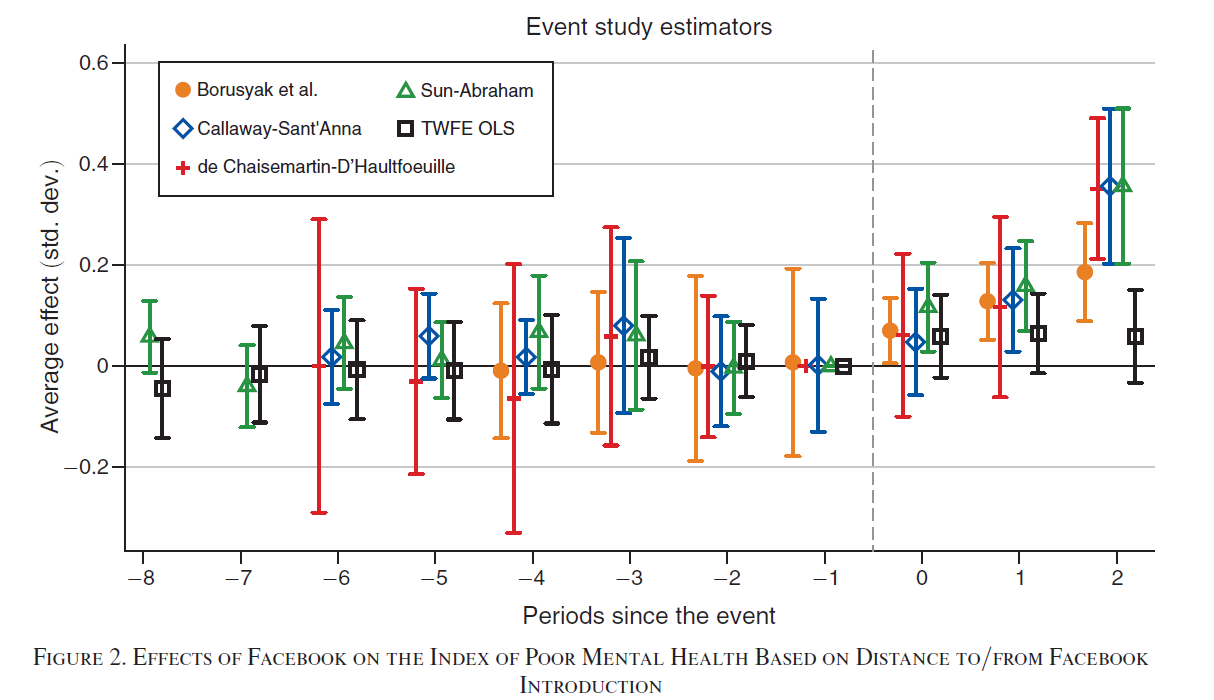
\includegraphics[width=0.75\linewidth]{Figuras/braghieri-salud-mental-resultados.png}
    \end{figure}        
\begin{itemize}
    \item Facebook empeora la salud mental: $+0.085$ desv. estándar.
    \item Impacto comparable al 22\% del efecto de perder el empleo.
    \item 24\% del aumento en depresión severa puede explicarse por Facebook.
\end{itemize}
\end{frame}


\begin{frame}{Ejemplo (2): \citet{kleven2019children}}
	\begin{itemize}\setlength{\itemsep}{1em}
	\item Diferencias importantes entre hombres y mujeres en ingresos laborales, participación laboral, y horas trabajadas (entre otros).
	%\pause
	\item Parte de la literatura se ha enfocado en identificar si estas diferencias se explican por discriminación, preferencias, normas sociales, patrones de acumulación de capital humano, etc.
	%\pause
	\item \citet{kleven2019children} estudian el efecto de tener hijos sobre la carrera de las mujeres.
	\end{itemize}	
\end{frame}


\begin{frame}{Estrategia de identificación}
	\begin{itemize}\setlength{\itemsep}{1em}
		\item Usan el momento del nacimiento del primer hijo para estudiar los efectos de este ``evento'' sobre diferentes resultados laborales: ingresos, horas trabajadas, y participación laboral.
        \vspace{0.5em}
		\begin{itemize}
			\item Se comparan hombres y mujeres antes y después del nacimiento del primer hijo.
			\item Diferentes parejas tienen el primer hijo a diferentes edades (diferentes momentos en la carrera).	
		\end{itemize}
		%\pause
		\item Construyen un panel de individuos con datos administrativos de Dinamarca entre 1980 y 2013.
		%\pause
		\item Identifican parejas para las cuáles hay información de al menos 5 años antes \textbf{del nacimiento del primer hijo} y 10 años después.
	\end{itemize}
\end{frame}


\begin{frame}{Especificación econométrica}
\begin{itemize}\setlength{\itemsep}{1em}
	\item Para cada individuo $i$ en el año $s$, definimos $t=0$ como el año en que nace el primer hijo ($t=-5,...,0,...10$ indica el tiempo (años) relativo al evento).
	\smallspace
	\begin{align*}
	Y_{ist}^g = \sum_{j\neq-1} \textcolor{brown}{\tau_j^{g}} \mathbf{1}\{j=t\} + \sum_{k} \beta_k^{g} \mathbf{1}\{k=age_{is}\} + \eta^g_s + e^g_{ist}
	\end{align*}
    %\pause
	\item $\mathbf{1}[k=age_{is}]$ son \textit{dummies} de edad, y $\eta^g_s$ son efectos fijos de año.
	\smallspace
	%\pause
	\item Se estima un modelo diferente para hombres ($g=m$) y mujeres ($g=w$). La \textit{``penalidad''} de tener un hijo es: 
	\begin{align*}
	    	P_{t} = \frac{\textcolor{brown}{\hat{\tau}^m_t} - \textcolor{brown}{\hat{\tau}^w_t}}{\EX[\hat{Y}^w_{ist}|t]}. 
	\end{align*}
\end{itemize}	
\end{frame}


\begin{frame}[plain]
	\begin{figure}[H]
		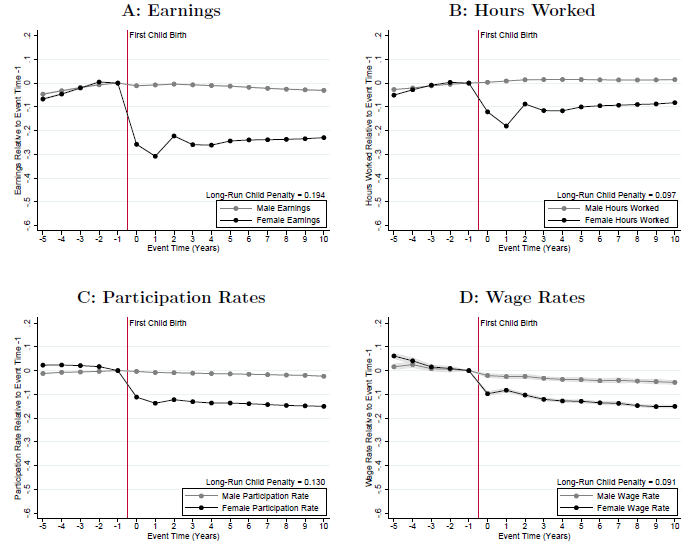
\includegraphics[width=7cm, height=7cm, keepaspectratio]{Figuras/child-penalty-evento-genero.png}
	\end{figure}
	\begin{enumerate}
		\vspace{-0.2cm}
		\item $\downarrow$ \textbf{ingresos} ($\approx -30\%$ en $t=0$) y \textbf{salario por hora} ($\approx -10\%$ en $t=0$).
		\item $\downarrow$ \textbf{horas trabajadas} ($\approx -12\%$ en $t=0$).
		\item $\downarrow$ \textbf{participación laboral} ($\approx -12\%$ en $t=0$). 
	\end{enumerate}
\end{frame}

%%%%%%%%%%%%%%%%%%%%%%%%%%%%%%%%%%%%%%%%%%%%%%%%%%%%%%%%%%%%%%
%%%%%%%%%%%%%%%%%%%%%%%%%%%%%%%%%%%%%%%%%%%%%%%%%%%%%%%%%%%%%%
%BIBLIOGRAPHY
\nobibliography{references}

\end{document}